\section{La transform\'ee de Fourier sur $\plone$}
\subsection{Les principaux espaces de suites et les r\`{e}gles de calcul}
\begin{definition}[Espaces de suites]
\begin{enumerate}[label=(\roman*)]
\item  $\plone$ l' espace des suites sommables  c' est-\`{a}-dire des suites $u$ qui v\'{e}rifient:
$$
\sum_{n=-\infty}^\infty |u_{n}|<+\infty,
$$
on note
$$
\Vert u\Vert_{1}=\sum_{n\in \zset}|u_{n}|
$$
qui est une norme sur l'espace des suites sommables.
\item On note $\pltwo$ l'espace des suites d'\'{e}nergie finie c'est-\`{a}-dire des suites $u$ qui v\'{e}rifient:
$$
\sum_{n\in \zset}|u_{n}|^{2}<+\infty,
$$
et on note
$$
\Vert u\Vert_{2}=\left(\sum_{n\in \zset}|u_{n}|^{2}\right)^{\frac{1}{2}}
$$
qui d\'efinit d'une norme sur l'espace des suites d'\'{e}nergie finie.
\item On note $\plinfty$ l'espace des suites born\'{e}es c'est-\`{a}-dire des suites $u$ qui v\'{e}rifient:
$$
\sup_{n \in \zset} |u_{n}| < \infty \eqsp,
$$
et on note
$$
\Vert u\Vert_{\infty}=\sup_{n\in \zset}\{|u_{n}|\}
$$
qui d\'efinit une norme sur l'espace des suites born\'{e}es.
\end{enumerate}
\end{definition}
\begin{lemma}
$$
\plone \subset \pltwo \subset \plinfty .
$$
\end{lemma}
\begin{proof}
Nous allons seulement prouver les inclusions:
\begin{enumerate}
\item $\plone \subset \pltwo$ : Soit $u\in \plone$ Soit $E\subset \zset$ d\'{e}fini par $E=\{n\ :\ |u_{n}|>1\}. \mathrm{L}$'ensemble $E$ est forc\'{e}ment fini, sinon $u$ aurait une somme infinie. Et on a
$$
\sum_{n \in \zset} |u_{n}|^{2}=\sum_{n \in \zset} |u_{n}|^{2}+\sum_{n \in \zset} |u_{n}|^{2}\leq\sum_{n \in E} |u_{n}|^{2}+\sum_{n \not \in E}|u_{n}|
$$
La derni\`{e}re in\'{e}galit\'{e} vient du fait que si $|x|\leq 1$ alors $|x|^{2}\leq|x|$. Or le premier terme de la derni\`{e}re somme est fini car $E$ est fini. Le second est fini aussi car $u$ est sommable. Donc $u\in \pltwo$
\item $\pltwo\subset \plinfty$ : Il est clair que si $u$ n'est pas born\'{e}e alors elle $\mathrm{a}$, par exemple, une infinit\'{e} de termes sup\'{e}rieurs \`{a} 1 en module. Les $|u_{n}|^{2}$ ne pourraient donc pas \^{e}tre sommables.
\end{enumerate}
\end{proof}
\begin{definition}[Convolution discr\`ete]
Si $u$ et $v$ sont des suites, on appelle produit de convolution de $u$et $v$ la suite d\'{e}finie par (si la somme a un sens):
$$
(u*v)_{n}=\sum_{m\in \zset}u_{m}v_{n-m}.
$$
\end{definition}
On v\'erifie de fa\c{c}on imm\'ediate que le produit de convolution est commutatif, lin\'{e}aire et associatif.
Nous donnons dans la proposition suivante les r\`{e}gles qui disent, suivant les espaces auxquels appartiennent $u$ et $v$, l'espace dont  $u*v$ et $u.v$ (produit terme \`{a} terme des deux suites) est \'el\'ement.

\begin{lemma}
\begin{enumerate}
\item Si $u\in \plone$et $v\in \olinfty$, alors $u.v\in \plone$ et
$$
\Vert u.v\Vert_{1}\leq\Vert u\Vert_{1}\Vert v\Vert_{\infty}
$$
\item Si $u\in \pltwo$ et $v\in \pltwo$, alors $u.v\in \plone$ et
$$
\Vert u.v\Vert_{1}\leq\Vert u\Vert_{2}\Vert v\Vert_{2}
$$
\end{enumerate}
\end{lemma}
\begin{proof}
La preuve \'el\'ementaire est laiss\'ee au lecteur.
\end{proof}
Nous obtenons ansi les r\`{e}gles de convolution que nous r\'esumons tableau suivant se lit comme suit, si $u$ appartient \`{a} un espace index de ligne et $v$ se trouve dans l'espace index de colonne, alors $u*v$ se trouve dans l'espace inscrit dans la case correspondante. Par exemple, si $u\in \plone$ et $v\in \plinfty$ alors $u*v\in \plinfty$ Si la case contient un tiret $(-)$ alors l'op\'{e}ration est a priori impossible (la s\'erie  peut ne pas avoir de sens). Et on a aussi \`{a} chaque fois, $\Vert u*v\Vert_{\gamma}\leq\Vert u\Vert_{\alpha}\Vert v\Vert_{\beta}$ (o\`{u} les normes $(y, \beta)$ et $\gamma$ sont les normes index de colonne, ligne et norme dans la case index\'{e}e respectivement. Par exemple $\Vert u*v\Vert_{\infty}\leq\Vert u\Vert_{1}\Vert v\Vert_{\infty}$
\begin{center}
\begin{tabular}{|l|l|l|l|}
\hline
\multicolumn{1}{|l|}{$*$}&	\multicolumn{1}{|l|}{ $\plone$}&	\multicolumn{1}{|l|}{ $\pltwo$}&	\multicolumn{1}{|l|}{ $\plinfty$}	\\
\hline
\end{tabular}


\begin{tabular}{|l|l|l|l|}
\hline
\multicolumn{1}{|l|}{$\plone$}&	\multicolumn{1}{|l|}{ $\plone$}&	\multicolumn{1}{|l|}{ $\pltwo$}&	\multicolumn{1}{|l|}{ $\plinfty$}	\\
\hline
\multicolumn{1}{|l|}{ $\pltwo$}&	\multicolumn{1}{|l|}{ $\pltwo$}&	\multicolumn{1}{|l|}{ $\plinfty$}&	\multicolumn{1}{|l|}{}	\\
\hline
\multicolumn{1}{|l|}{ $\plinfty$}&	\multicolumn{1}{|l|}{ $\plinfty$}&	\multicolumn{1}{|l|}{}&	\multicolumn{1}{|l|}{}	\\
\hline
\end{tabular}

\end{center}

\subsection{La Transform\'{e}e de Fourier \`{a} temps Discret (TFTD)}

\begin{definition}
Si $u$ est une suite sommable $(u\in \plone)$ , on appelle Transform\'{e}e de Fourier \`{a} temps Discret ( TFtD en abr\'{e}g\'{e}), la fonction d\'{e}finie sur l'intervalle $\coint{-1/2,1/2}$
et que l'on note soit $\hat{u}$ soit $\TFA{u}$
$$
\hat{u}(\nu)=\sum_{n\in \zset}u_{n}\rme^{-2\rmi\pi n \nu }
$$
\end{definition}
Quand $u\in \plone$,$\hat{u}$ est une fonction continue et admet une limite en $1/2$ \'{e}gale \`{a} sa valeur en $-1/2$
(elle est donc continue m\^{e}me si on la consid\`erre comme une fonction d\'{e}finie sur $\rset$)

Le fait que la d\'{e}finition ait un sens d\'{e}coule du fait que $u$ est suppos\'{e}e sommable. Le fait que $\hat{u}$ soit continue utilise le th\'{e}or\`{e}me de convergence domin\'{e}e.

Pour$m \in \nset$, on note $\theta_m$ l'op\'erateur de retard, d\'efini pour une suite $u= \sequence{u}[n][\nset]$ par
\begin{equation}
(\theta_m u)_n = u_{n-m} \eqsp.
\end{equation}
\begin{proposition}[Propri\'{e}t\'{e}s de la TFtD]
\label{prop:propriete-TFTD}
\begin{enumerate}[label=(\roman*)]
\item $\TFA{\theta_n u}(\nu)= \rme^{- 2 \rmi \pi m \nu} \TFA{u}(\nu)$ pour tout $\nu \in \coint{-1/2,1/2}$.
\item $\TFA{\delta}(\nu) = 1$ pour tout $\nu \in \coint{-1/2,1/2}$.
\item Si $u, v \in \plone$, $\TFA{u * v}= \TFA{u} \, \TFA{v}$
\item Si $u \in \plone$ et $v \in \plinfty$, $\TFA{u \cdot v}=\TFA{u}*\TFA{v}$
\item Si $u \in \plone$, $\nu_0 \in \coint{-1/2,1/2}$, pour tout $\nu \in \coint{-1/2,1/2}$,
$\TFA{ u \cdot e_{\nu_0}}(\nu)= \TFA{u}(\nu - \nu_0)$, o\`u $e_{\nu_0}(n) = \rme^{-2 \rmi \pi \nu_0 n}$.
\item Si $u$ est r\'{e}elle, alors $\TFA{u}(-\nu) = \TFAC{u}(\nu)$.
\end{enumerate}
\end{proposition}
\begin{proof}
Ces propri\'et\'es sont \'el\'ementaires et la preuve est laiss\'ee au lecteur.
\end{proof}

\begin{definition}[Syst\`eme ln\'eaire invariant dans le temps (SLI)]
$T$ est un $SLI$ qui transforme une suite born\'{e}e en une suite born\'{e}e, alors on sait que $T$ poss\`{e}de une r\'{e}ponse impulsionnelle sommable  que l'on note $h.$

Si $u$ est une suite sommable (donc born\'{e}e) et $v=T(u)$ la sortie qui lui est associ\'{e}e par $T$ alors on a :

1. La r\'{e}ponse (ou le gain) fr\'{e}quentielle duSLIT est la transform\'{e}e de Fourier de $h.$ 2. La suite $v$ est sommable, car $h*v\in \plone$ d'apr\`{e}s les r\`{e}gles de calcul.

3. Et
$$
\hat{v}=\hat{h}\hat{u}.
$$
D}'apr\`{e}s les propri\'{e}t\'{e}s de la TFtD}.

Ainsi, un $SLI$ agit sur la transform\'{e}e de Fourier de l'entr\'{e}e par multiplication de celle-ci, point \`{a} point par sa r\'{e}ponse fr\'{e}quentielle}.

\begin{proof}
Commencons par remarquer que les suite $u, v$ et $h$ ont bien toutes une transform\'{e}e de Fourier \`{a} temps discret, car elles sont toutes sommables.

La seule chose qui reste \`{a} montrer est la premi\`{e}re affirmation. Soit donc une onde de Fourier de fr\'{e}quence $\nu$, son terme g\'{e}n\'{e}ral est $e^{2i\pi\nu n}$ La sortie qui lui est associ\'{e}e est, par d\'{e}finition de la r\'{e}ponse fr\'{e}quentielle, de terme g\'{e}n\'{e}ral $C(\nu)e^{2i\pi 1/n}$, o\`{u} $C(\nu)$ est la r\'{e}ponse fr\'{e}quentielle.

Or la valeur en z\'{e}ro de la r\'{e}ponse de $T$ \`{a} l'harmonique complexe de Fourier est donn\'{e}e par (convolution entre $h$ et l'harmonique complexe de Fourier) :
$$
\sum_{m\in \zset}h_{m}e^{2i\pi\nu(0-m)}=\hat{h}(\nu)=C(\nu)
$$
La premi\`{e}re \'{e}galit\'{e} vient de la d\'{e}finition de la TFtD, et la seconde de la d\'{e}finition de la r\'{e}ponse fr\'{e}quentielle (la valeur en z\'{e}ro de la sortie associ\'{e}e \`{a} une onde de Fourier).
\end{proof}

\section{La transform\'ee de Fourier sur $\pltwo$}
Nous avons d\'{e}fini la TFTD pour les suites sommables. Il est possible d'\'{e}tendre cette d\'{e}finition aux suites $\pltwo$ (rappelons que $\plone \subset \pltwo$).

\begin{theorem}[Extension \`{a} $\pltwo$ et \'{e}galit\'{e} de Parseval]
Il existe un unique prolongement isom\'etrique  $\TF$ de $\pltwo$ \mapsto $\ltwo(\coint{-1/2,1/2})$ qui co\"incide avec la TFTD sur $\lone$. Pour tout $u \in \pltwo$
$\Vert\hat{u}\Vert_{2}=\Vert u\Vert_{2}$, soit plus explicitement}:
$$
\int_{-\frac{1}{2}}^{\frac{1}{2}}|\TFA{u}(\nu)|^{2} \rmd\nu=\sum_{n\in \zset}|u_{n}|^{2}
$$
\end{theorem}
\begin{proof}
Montrons tout d'abord que $\TF$ d\'efini une isom\'etrie sur $\plone$. Soit $u \in \plone$. Nous avons
\begin{align*}
\int_{-1/2}^{1/2} |\hat{u}(\nu)|^2 \rme \nu &= \int_{-1/2}^{1/2} \left| \sum_{k \in \zset} u_k \rme^{-2 \rmi \pi k \nu} \right|^2 \rmd \nu \\
&= \int_{-1/2}^{1/2} \sum_{k,l=-\infty}^{\infty} u_k \bar{u}_l \rme^{-2 \rmi \pi (k-l)} \rmd \nu \\
&= \sum_{k,l \in \zset} u_k \bar{u}_l \int_{-1/2}^{1/2} \rme^{- 2 \rmi \pi (k-l) \nu} \rmd \nu \\
&= \sum_{k=-\infty}^{\infty |u_k|^2 \eqsp.
\end{align*}
La permutation des int\'egrales et des sommes est justifi\'ee par application du th\'eor\`eme de Fubini car
\[
\int_{-1/2}^{1/2} \sum_{k,l \in \zset} |u_k| |u_l| \rmd \nu < \infty \eqsp.
\]
D'autre part, $\plone$ est dense dans $\pltwo$: si $u \in \pltwo$ alors pour tout $N \in \nset$, la suite $u^N$ d\'efinie par
$u^N_k = u_k$ si $|k| \leq N$ et $u^N_k= 0$ sinon est \'el\'ement de $\lone(\zset)$ et $\| u - u^N \|_2^2 = \sum_{|k| > N} |u_k|^2 \to 0$. La preuve d\'ecoule de \Cref{theo:prolongement-isometrie}
\end{proof}
Les propri\'{e}t\'{e}s de \Cref{{prop:propriete-TFTD}} restent encore vraies en prenant $u$ et $v$ dans $\pltwo$, \`{a} des d\'{e}tails pr\`{e}s : il faut prendre $u\in \pltwo$ et $v\in \plone$, sinon la convolution de $u$ et $v$ n'est a priori ni dans $\plone$ ni dans $\pltwo$

\begin{theorem}[Inversion de la TFtd]
Si $u\in \pltwo$ est une suite d}'\'{e}nergie finie et $\TFA{u}=\hat{u}$ sa TFtD alors on a, pour tout $n \in \zset$,
$$
u_{n}=\int_{-\frac{1}{2}}^{\frac{1}{2}}\hat{u}(\nu)\rme^{2\rmi \pi \nu} \rmd \nu
$$
o\`u, de fa\c{c}on plus concise $\TFAC{\TFA{u}}=u$.
\end{theorem}
\begin{proof}
Consid\'erons tout d'abord $u \in \plone$. Nous avons
\begin{align*}
\int_{-1/2}^{1/2} \hat{u}(\nu) \rme^{2 \rmi \pi \nu n} \rmd \nu &= \int_{-1/2}^{1/2} \left( \sum_{k \in \zset} u_k \rme^{-2 \rmi \pi k \nu}\right) \rme^{2 \rmi \pi n \nu} \rmd \nu \\
&= \sum_{k \in \zset} u_k \int_{-1/2}^{1/2} \rme^{-2 \rmi \pi (k-n) \nu} \rmd \nu = u_n \eqsp.
\end{align*}
La permutation de l'int\'egrale et du signe somme est justifi\'e car
\[
\int_{-1/2}^{1/2} \sum_{k \in \zset} |u_k| \rmd \nu < \infty \eqsp.
\]
Soit maintenant $u \in \pltwo$ et $u^N$ la suite tronqu\'ee, $u^N_k = u_k$ pour $|k| \leq N$, $u_k^N=0$ sinon. En notant
$\nu \mapsto e_n(\nu)= \rme^{-2 \rmi \pi n \nu }$, nous avons
\begin{align*}
\int_{-1/2}^{1/2} \hat{u}(\nu) \rme^{2 \rmi \pi n \nu} &= \pscal{u}{e_n} \\
&= \lim_{N \to \infty} \pscal{u^N}{e_n}= \lim_{N \to \infty} u_n^N = u_n \eqsp.
\end{align*}
\end{proof}
On a vu que la r\'{e}ponse fr\'{e}quentielle d'un SLI est la TFtD de sa r\'{e}ponse impulsionnelle. Le th\'{e}or\`{e}me d'inversion nous permet de retrouver la r\'{e}ponse impulsionnelle \`{a} partir de sa r\'{e}ponse fr\'{e}quentielle. Ainsi, pour d\'{e}finir un SLI, il suffit de donner soit sa r\'{e}ponse impul- sionnelle (ce que nous savions d\'{e}j\`{a}) ou sa r\'{e}ponse fr\'{e}quentielle (qui permet de retrouver la r\'{e}ponse impulsionnelle gr\^{a}ce au th\'{e}or\`{e}me d'inversion).

\subsection{D\'{e}croissance \`{a} l'infini et r\'{e}gularit\'{e}}
Nous savons d\'{e}j\`{a} que si $u$ est sommable alors $\hat{u}$ est continue. La sommabilit\'{e} est une forme de d\'{e}croissance \`{a} l'infini (pour les suites, cela implique m\^{e}me que $u_{n}$ tende vers $0$ \`{a} l'infini). Le th\'{e}or\`{e}me suivant dit que plus la suite $u\mathrm{d}\acute{\mathrm{e}}\mathrm{c}\mathrm{r}\mathrm{o}\hat{\mathrm{l}}\mathrm{t}$ rapidement \`{a} l'infini, plus sa TFtD est r\'{e}guli\`{e}re.

\begin{theorem}[D\'{e}croissance \`{a} l'infini et r\'{e}gularit\'{e} de la TFtD]
Soit $k\geq 0$ un entier, on a :
\begin{enumerate}[label=(\roman*)]
\item Si $(\sum_{n\in \zset}|n|^{k}|u_{n}|<\infty$ alors $\hat{u}$ est $k$ fois continuement d\'{e}rivable. 
\item Notons $v^{(k)}$ la suite de terme g\'{e}n\'{e}ral
$$
v_{n}^{(k)}=(-2 \rmi\pi n)^{k}u_{n} \eqsp.
$$
Si $v^{(k)} \in \pltwo$, la TFtD de $v^{(k)}$ est $\TFA{v^{(k)}}=\TFA{u}^{(k)}$ (la d\'{e}riv\'{e}e} $k$-i\`{e}me de $\TFA{u}$ 
\end{enumerate}
\end{theorem}
\begin{proof}
La preuve est \'el\'mentaire et laiss\'ee au lecteur
\end{proof}
\section{Transform\'{e}e de Fourier Discr\`{e}te ou TFD}
La Transform\'{e}e de Fourier discr\`{e}te est la transformation de Fourier pour les signaux d\'{e}finis sur un ensemble $\{0,\ \ldots,\ N-1\}$. Les suites d\'{e}finies sur cet ensemble sont toutes sommables, born\'{e}es et d'\'{e}nergie finie (car elles sont \`{a} support fini).

\begin{definition}[Transform\'{e}e de Fourier Discr\`{e}te]
Si $u$ est une suite finie d\'{e}finie sur $\{0,\ \ldots,\ N-1\}$, on note $\hat{u}$  sa Transform\'{e}e de Fourier Discr\`{e}te} (TFD en abr\'{e}g\'{e}}) d\'{e}finie, elle aussi sur} $\{0,\ \ldots,\ N-1\}$, pour tout $k\in\{0,\ \ldots,\ N-1\}$
$$
\hat{u}_k=\sum_{n=0}^{N-1} u_{n}\rme^{-2\rmi\pi \frac{k}{N}n}
$$
\end{definition}
Notons $W_N= \rme^{-2 \rmi \pi /N}$ et pour $k \in \{0,\dots,N-1}$, $E_k= [W_N^{k \cdot 0}, \dots, W_N^{k \cdot (N-1)}]'$.
Nous avons pour tout $k,l \in \{0, \dots, N-1\}$, $E_k^H E_l= N \delta_{k,l}$ où $\delta_{k,l}$ est le symbole de Kronecker.
Nous avons donc, en notant $U= [u_0, \dots, u_{N-1}]$,
\[
\hat{u}_k = E_k^H U \eqsp.
\]
\begin{theorem}[Inversion de la TFD]
Soit $u$ une suite d\'{e}finie sur $\{0,\ \ldots,\ N-1\}$ et $\hat{u}$ sa TFD on a, pour tout $n\in\{0,\ \ldots,\ N-1\}$
$$
u_{n}=\frac{1}{N}\sum_{k=0}^{n-1} \hat{u}_{k} \rme^{2 \rmi\pi\frac{k}{N}n} \eqsp.
$$
De plus,
\[
\sum_{k=0}^{N-1} |u_k|^2 = \frac{1}{N} \sum_{k=0}^{N-1} |\hat{u}_k|^2 \eqsp.
\]
\end{theorem}
\begin{proof}
Nous avons, comme les vecteurs $(E_k)_{k=0}^{N-1}$ sont orthogonaux.
\[
U = \sum_{k=0}^{N-1} \frac{E_k^H U}{E_k^H E_k} E_k = \frac{1}{N} \sum_{k=0}^{N-1} \hat{u}_k E_k \eqsp.
\]
D'autre part, 
\[
\sum_{k=0}^{N-1} |u_k|^2= \frac{1}{N}^2 \sum_{k=0}^{N-1} |\hat{u}_k|^2 E_k^H E_k= \frac{1}{N} \sum_{k=0}^{N-1} |U_k|^2 \eqsp.
\]
\end{proof}
Clairement, la TFD est une application lin\'eaire de $\cset^N$ \`a valeurs dans $\cset^N$.
Les autres propri\'et\'es de la TFD doivent être consid\'er\'es avec un peu de pr\'ecaution.
Remarquons tout d'abord la suite finie $u= \{u_0, \dots, u_{N-1}\}$ peut être prolong\'ee en une suite p\'eriodique de
p\'eriode $N$,
\begin{equation}\label{eq:periodisee}
\tilde{u}_n= u_{ n \pmod{N}} 
\end{equation}
Soit maintenant $m \in \zset$. Il est l\'egitime de consid\'erer
$$
\theta_m \tilde{u}_n = \tilde{u}_{n-m} = u_{ (n-m) \pmod{N} }
$$
Lorsque l'on applique l'op\'erateur retard $\theta_m$ à la suite p\'eriodis\'ee, nous obtenons de nouveau une suite p\'eriodique de p\'eriode $N$.
On peut donc calculer la TFD de cette suite, pour tout $k \in \{0,\dots,N-1\}$, nous avons
\begin{align*}
\sum_{n=0}^{N-1} u_{ (n-m) \pmod{N}} W_N^{nk} &= \sum_{n=0}^{N-1} \tilde{u}_{(n-m) \pmod{N}} W_N^{nk}= \sum_{\ell=-m}^{N-m-1} \tilde{u}_{\ell} W_N^{(\ell + m)k} \eqsp.
\end{align*}
Comme  $W_N^{(\ell +m)k}= W_N^{mk} W_N^{\ell k}$, nous avons
\[
\sum_{n=0}^{N-1} u_{ (n-m) \pmod{N}} W_N^{nk} = W_N^{mk} \sum_{\ell=-m}^{N-m-1} \tilde{u}_{\ell} W_N^{\ell k}= W_N^{mk} \hat{u}_k \eqsp,
\]
où nous avons utilis\'e que la suite $v_\ell= \tilde{u}_{\ell} W_N^{\ell k}$ est $N$-p\'eriodique et pour tout suite $w$ $N$-p\'eriodique et tout $m \in \zset$, $\sum_{\ell=-m}^{N-m-1} w_{\ell}= \sum_{\ell=0}^{N-1} w_\ell$.



\subsection{Lien entre TFD et TFtD}
La TFD est la seule transform\'{e}e de Fourier calculable sur ordinateur. La plupart des signaux naturels sont d\'{e}finis sur un espace \`{a} la fois infini et continu $(\rset$ pour le son, par exemple). La TFD s'int\'{e}resse \`{a} des signaux d\'{e}finis sur un espace fini et discret.  Dans cette partie nous allons voir comment une TFD peut permettre d'analyser un signal d\'{e}fini sur $\zset$, r\'{e}alisant ainsi un p,assage de l'infini au fini.

Evidemment, une TFD ne peut capturer toutes les caract\'{e}ristiques d'un signal quelconque, il nous faut restreindre notre \'{e}tude \`{a} des cas particuliers. Nous verrons : 
\begin{enumerate}
\item Cas d'une suite \`{a} support fini.
\item D\'{e}termination de la fr\'{e}quence d'une exponentielle complexe.
\item S\'{e}paration de la somme de deux exponentielle complexe (qui nous permettra de comprendre l'importance du fenêtrage)
\end{enumerate}

\subsubsection{Cas d'une suite \`{a} support fini}
Soit une suite $u$ d\'{e}finie sur $\zset$ \`{a} support fini. Sans perte de g\'{e}n\'{e}ralit\'{e}, quitte \`{a} la translater, on peut supposer qu'il existe un entier $N$ tel que, pour tout  $n\in \zset$, $u_{n}=0$ si $n<0$ ou $n\geq N$

Pour tout entier $M\geq N$ on consid\`{e}re la suite finie $v$ d\'{e}finie sur $\{0,\ \ldots,\ M-1\}$, pour tout $n\in\{0,\ \ldots,\ M-1\}$,
$$
v_{n}=u_{n}
$$
La suite finie $v$ est simplement la restriction de $u$ \`{a} l'ensemble $\{0,\ \ldots,\ M-1\}$. On appelle parfois $v$ la suite z\'{e}ro-padding \`{a} l'ordre $M$ de $u$. On ajoute des z\'{e}ros \`{a} la suite des \'{e}chantillons non nuls de $u$ pour obtenir une suite de taille $M$. Pour tout $k\in\{0,\ \ldots,\ M-1\}$, 
$$
\hat{v}(k)=\sum_{n\in\{0,\ldots,M-1\}}v_{n}\rme^{-2\rmi\pi \frac{k}{M}n}=\hat{u}(\frac{k}{M})
$$
o\`{u} $\hat{u}$ est la TFtD de $u$. la derni\`{e}re \'{e}galit\'{e} provient du fait que $u$ est nulle hors de $\{0,\ \ldots,\ N-1\}$ et donc hors de $\{0,\ \ldots,\ M-1\})$ .



\begin{figure}
  \centering
  % Requires \usepackage{graphicx}
  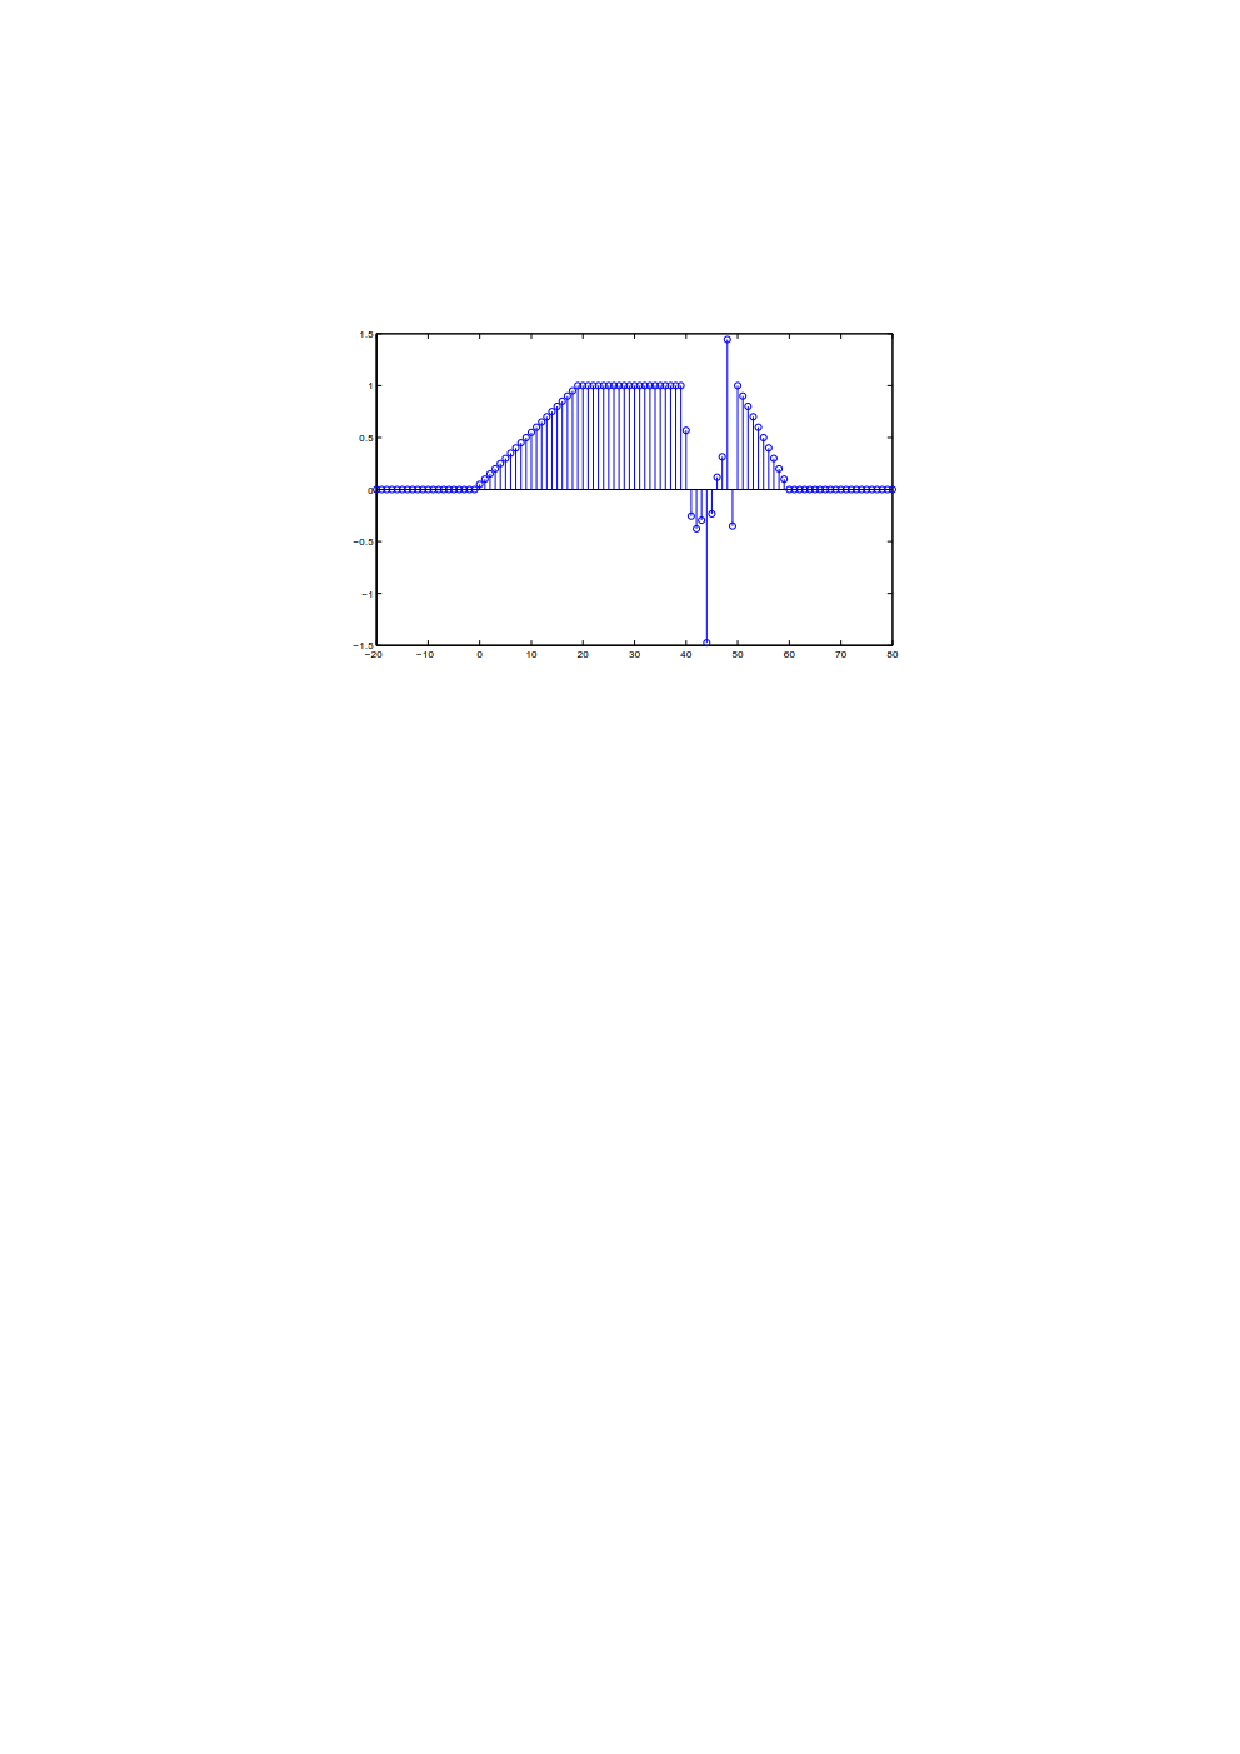
\includegraphics[width=0.6\textwidth]{Figures/Figure2-1}\\
  \caption{Un signal  \`a support fini}\label{fig:figure2-1}
\end{figure}

\begin{figure}
  \centering
  % Requires \usepackage{graphicx}
  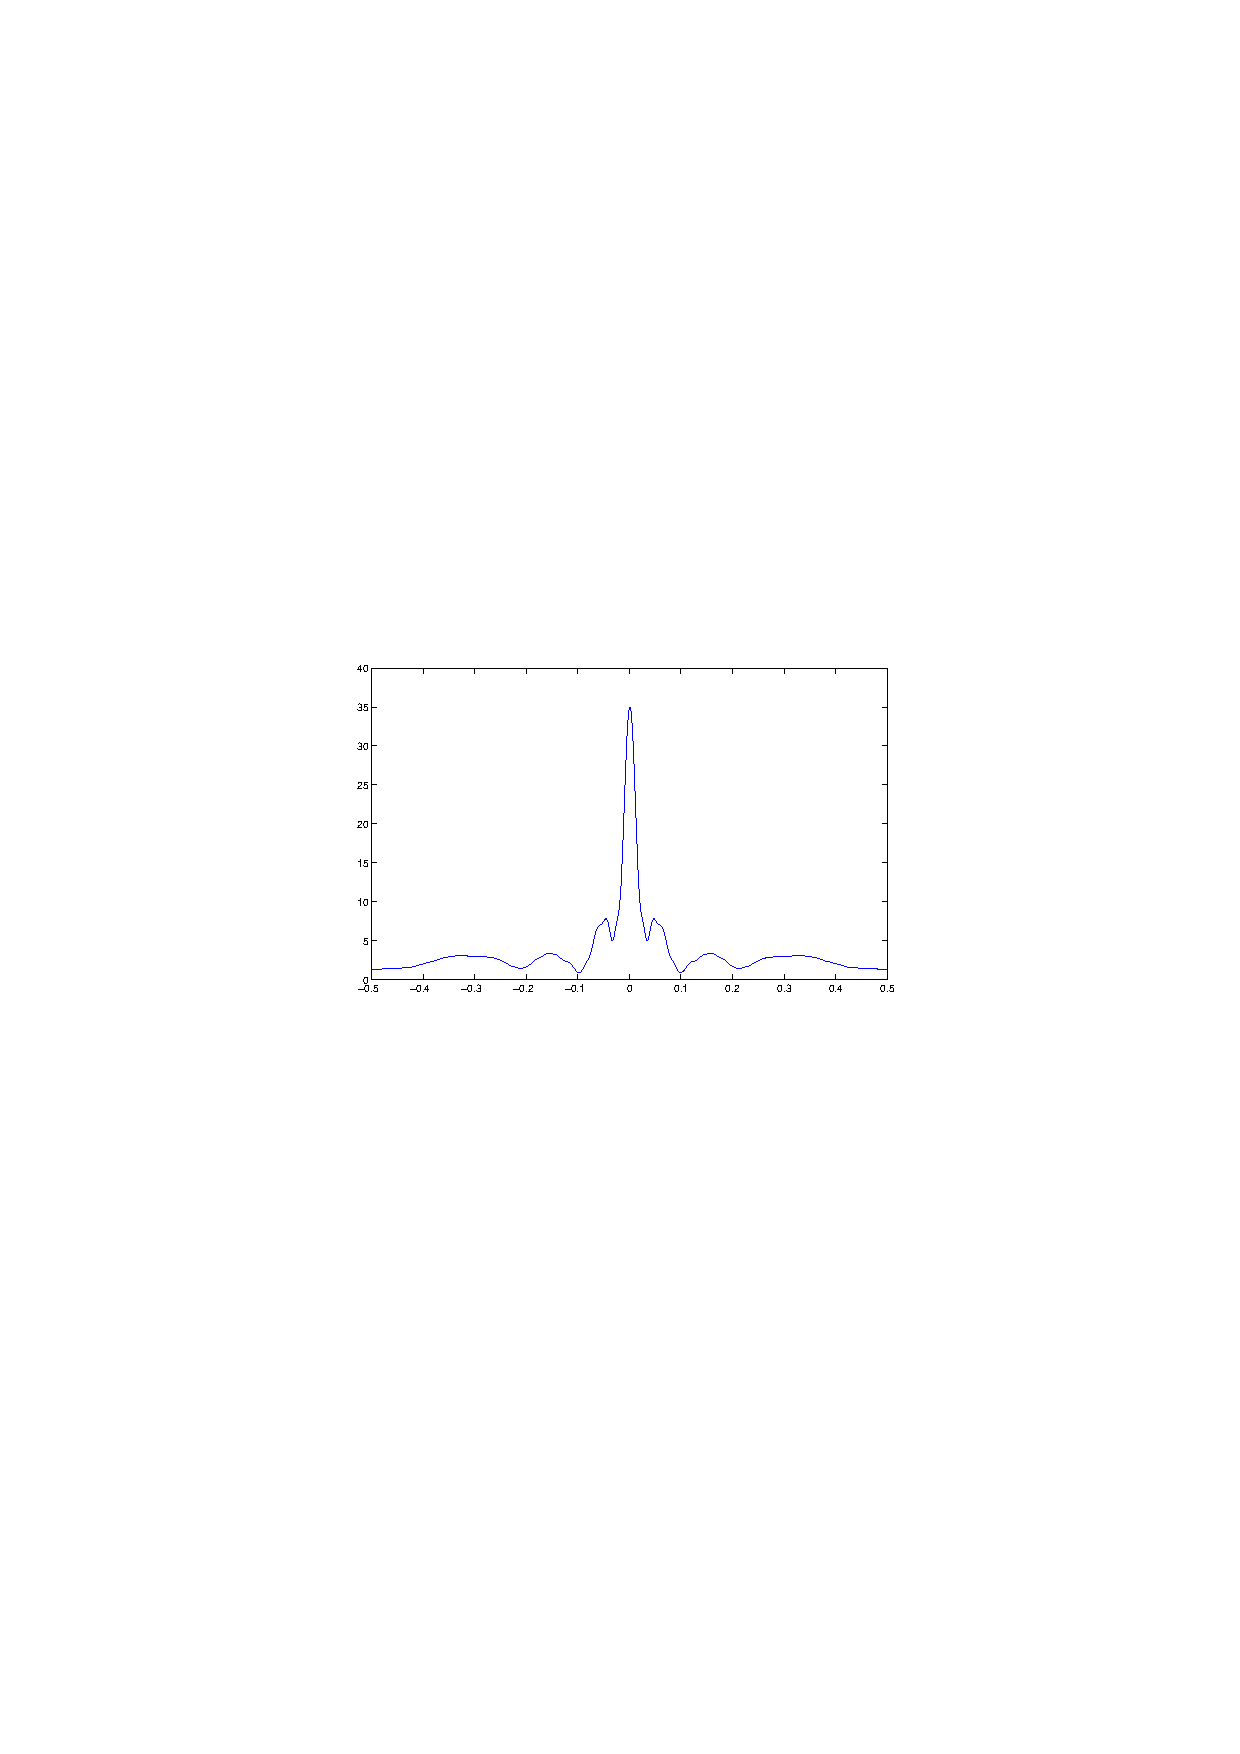
\includegraphics[width=0.6\textwidth]{Figures/Figure2-2}\\
  \caption{module de la TFtD du signal; comme le signal est r\'eel, le module de la TFtD est une fonction paire}\label{fig:figure2-2}
\end{figure}

\begin{figure}
  \centering
  % Requires \usepackage{graphicx}
  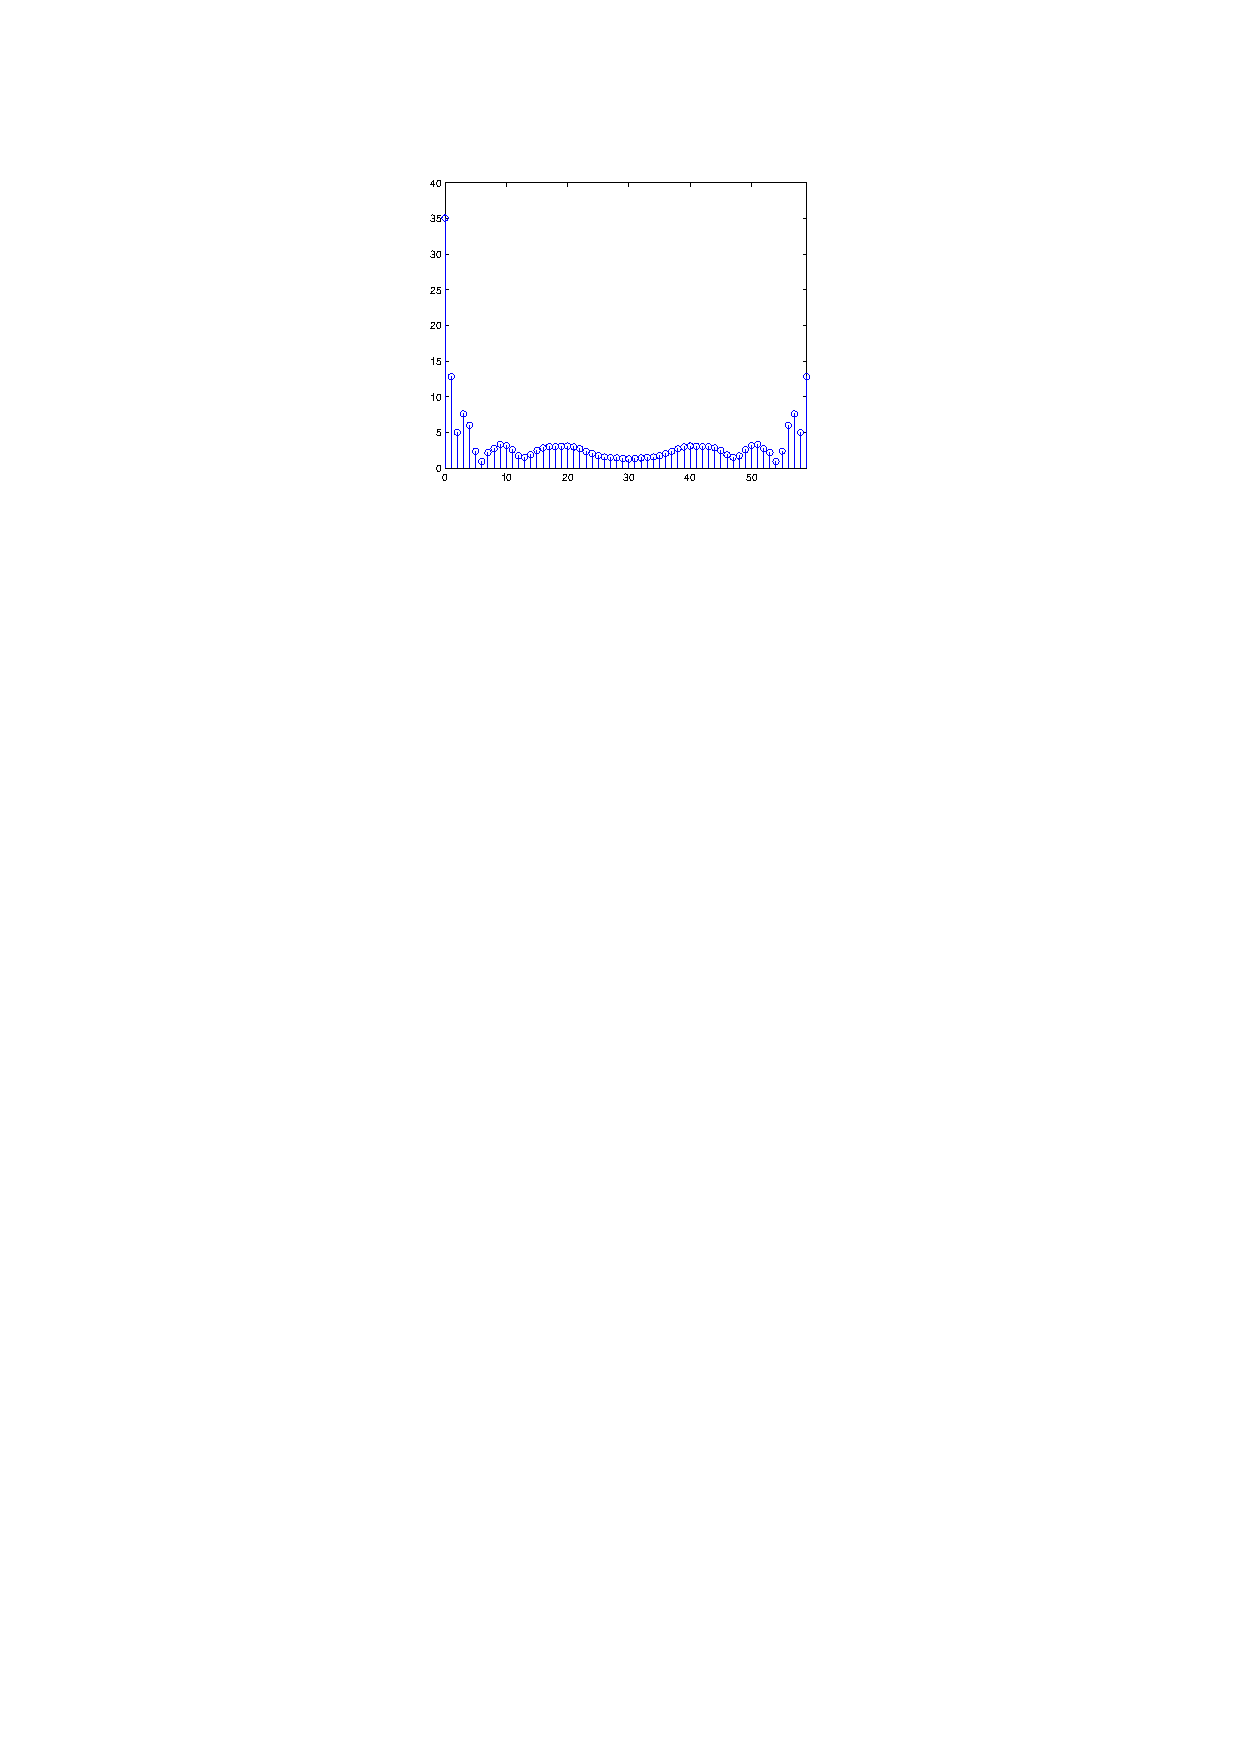
\includegraphics[width=0.6\textwidth]{Figures/Figure2-3}\\
  \caption{module de la TFD du signal}\label{fig:figure2-3}
\end{figure}

\begin{figure}
  \centering
  % Requires \usepackage{graphicx}
  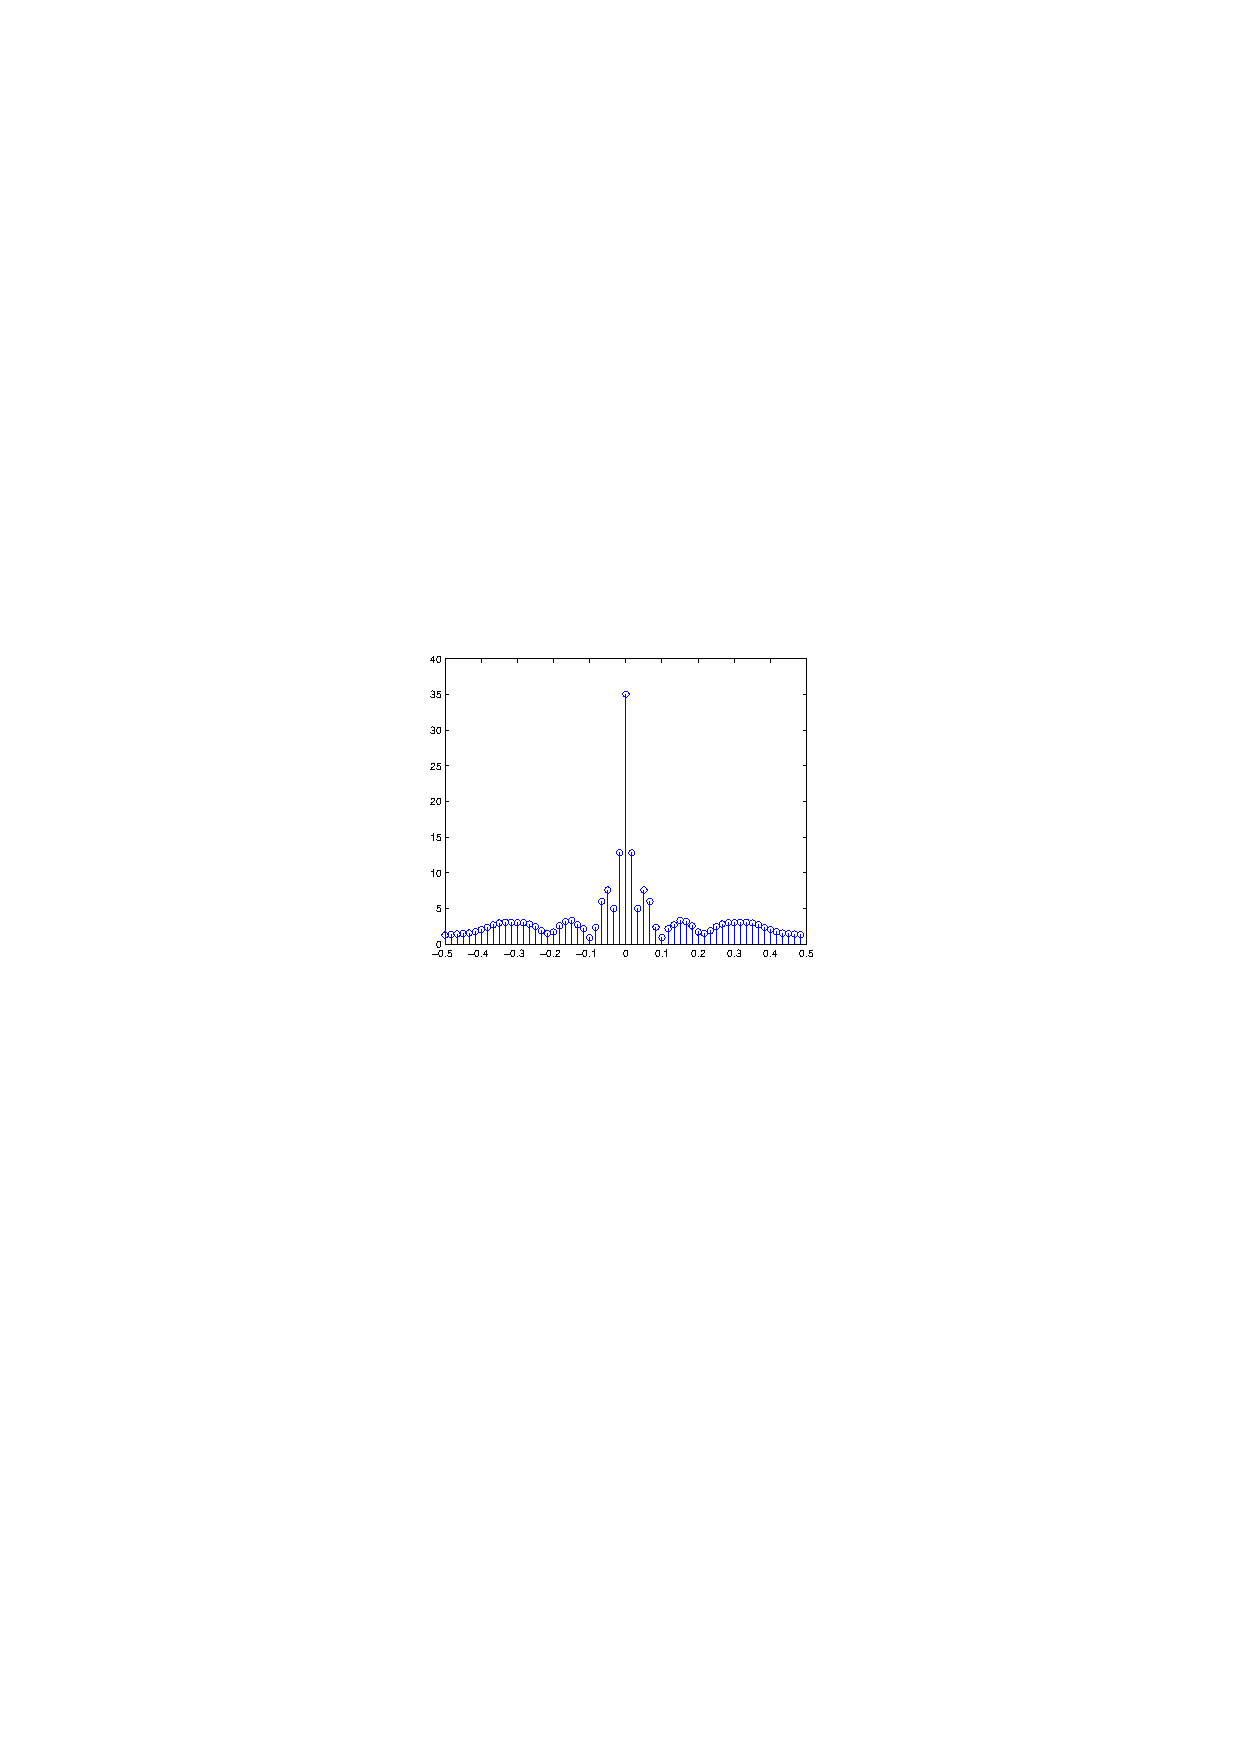
\includegraphics[width=0.6\textwidth]{Figures/Figure2-4}\\
  \caption{module de la TFD p\'eriodis\'e et remise \`a l'\'echelle}\label{fig:figure2-4}
\end{figure}

\subsubsection{Estimation d'une fr\'equence}
On se donne une onde $u_{n}=e^{2i\pi 1/0n}$ On voudrait d\'{e}terminer la fr\'{e}quence $\nu_{0}$ on ne se donnant le droit que d'observer les \'{e}chantillons $u_{0}, \ldots, u_{N}$. Pourquoi une telle contrainte? Dans un signal, musical par exemple, le contenu fr\'{e}quentiel \'{e}volue au cours du temps. \`{A} chaque changement de note, le signal contient des ondes de fr\'{e}quences diff\'{e}rentes. Si l'on veut, par exemple, transcrire un morceau de musique en notes, on ne peut pas se permettre une observation sur une trop longue p\'{e}riode car cela aurait pour effet de m\'{e}langer entre elles diff\'{e}rentes notes. La m\^{e}me chose vaut pour l'analyse d'un signal de parole o\`{u} l'on risque la confusion entre diff\'{e}rents phon\`{e}mes.

On note $u^{T}$ (pour `` $u$ Tronqu\'{e}e'') la suite d\'{e}finie sur $\zset$ \'{e}gale \`{a} $u$ sur $\{0,\ \ldots,\ N-1\}$ et nulle ailleurs. Ce sont les seules valeurs que nous nous donnons le droit d'utiliser pour d\'{e}terminer $\nu_{0}$. Sa TFtD est
$$
\forall\nu\in[-\frac{1}{2},\ \frac{1}{2}[,\ \mathcal{F}(u^{T})(\nu)=e^{-i\pi.(N-1)(1/-1/0)^{sin(N\pi(\nu-\nu_{0}))}}
$$
$$
sin(\pi(\nu-\nu_{0}))
$$
Le module de $\mathcal{F}(u^{T})$ et donn\'{e} \`{a} la figure 2.6.

Si on calcule une TFD d'ordre $M\geq N$, on sait que l'on va \'{e}chantillonner la TFtD de $u^{T}$ aux point $k/M$. Deux TFD d'ordres diff\'{e}rents sont donn\'{e}es aux figures 2.7 et 2.8.


Avec une} $TFD$ d}'ordre} $M$ on peut conna\^{i}tre la fr\'{e}quence de l'harmonique complexe} $\nu_{0}$ avec une pr\'{e}cision d}'au moins} $1/M.$
En effet, quelque soit $\nu_{0}$ il existe au moins un $k$ pour lequel $k/M$ s'approche \`{a} moins $1/M$ de $\nu_{0}.$

\begin{figure}
  \centering
  % Requires \usepackage{graphicx}
  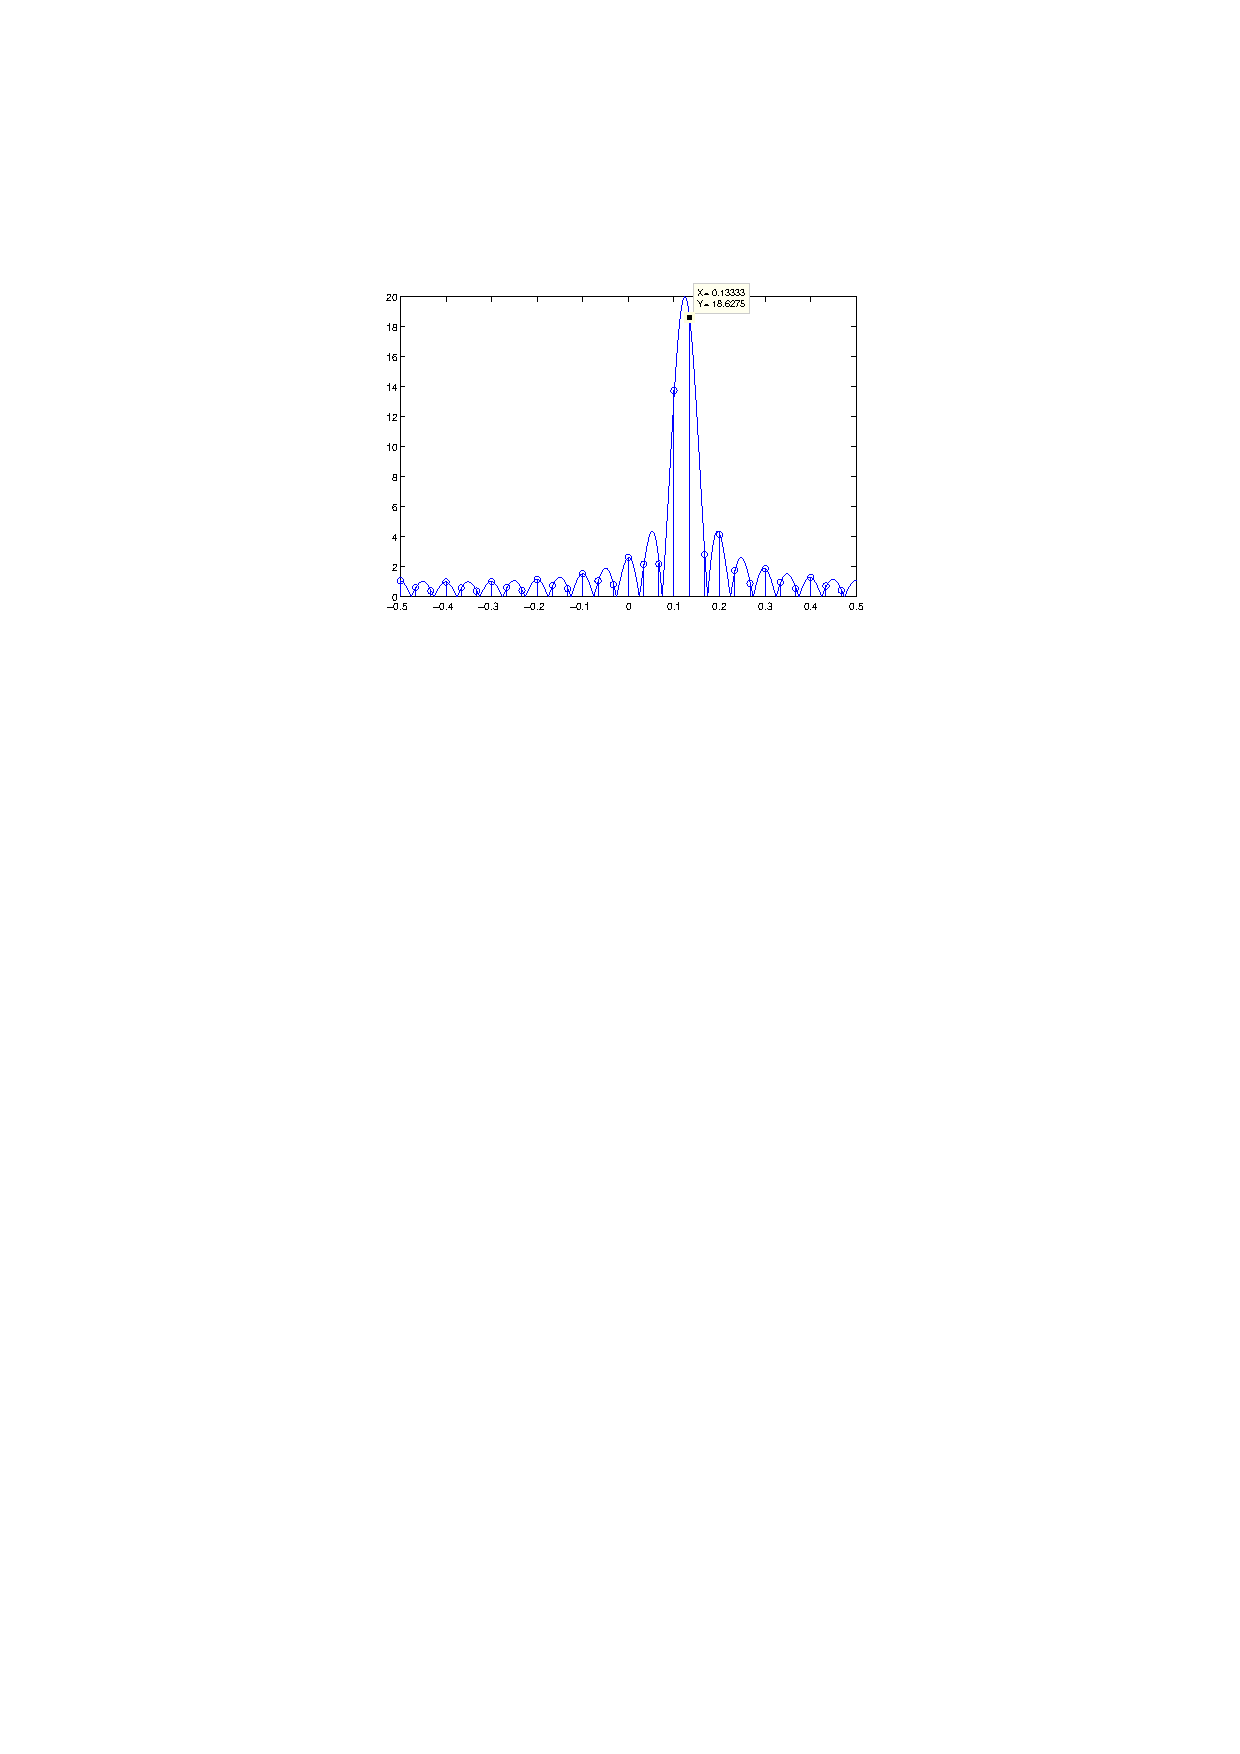
\includegraphics[width=0.6\textwidth]{Figures/Figure2-7}\\
  \caption{La TFD d'ordre 30 de l'harmonique complexe tronqu\'{e}e superpos\'{e}e \`{a} la TFtD. Le maximum de la TFD est atteint pour $k=4$, soit une fr\'{e}quence de $4/30=0$, 1333 et une erreur d'estimation de 0,01}\label{fig:figure2-7}
\end{figure}


\begin{figure}
  \centering
  % Requires \usepackage{graphicx}
  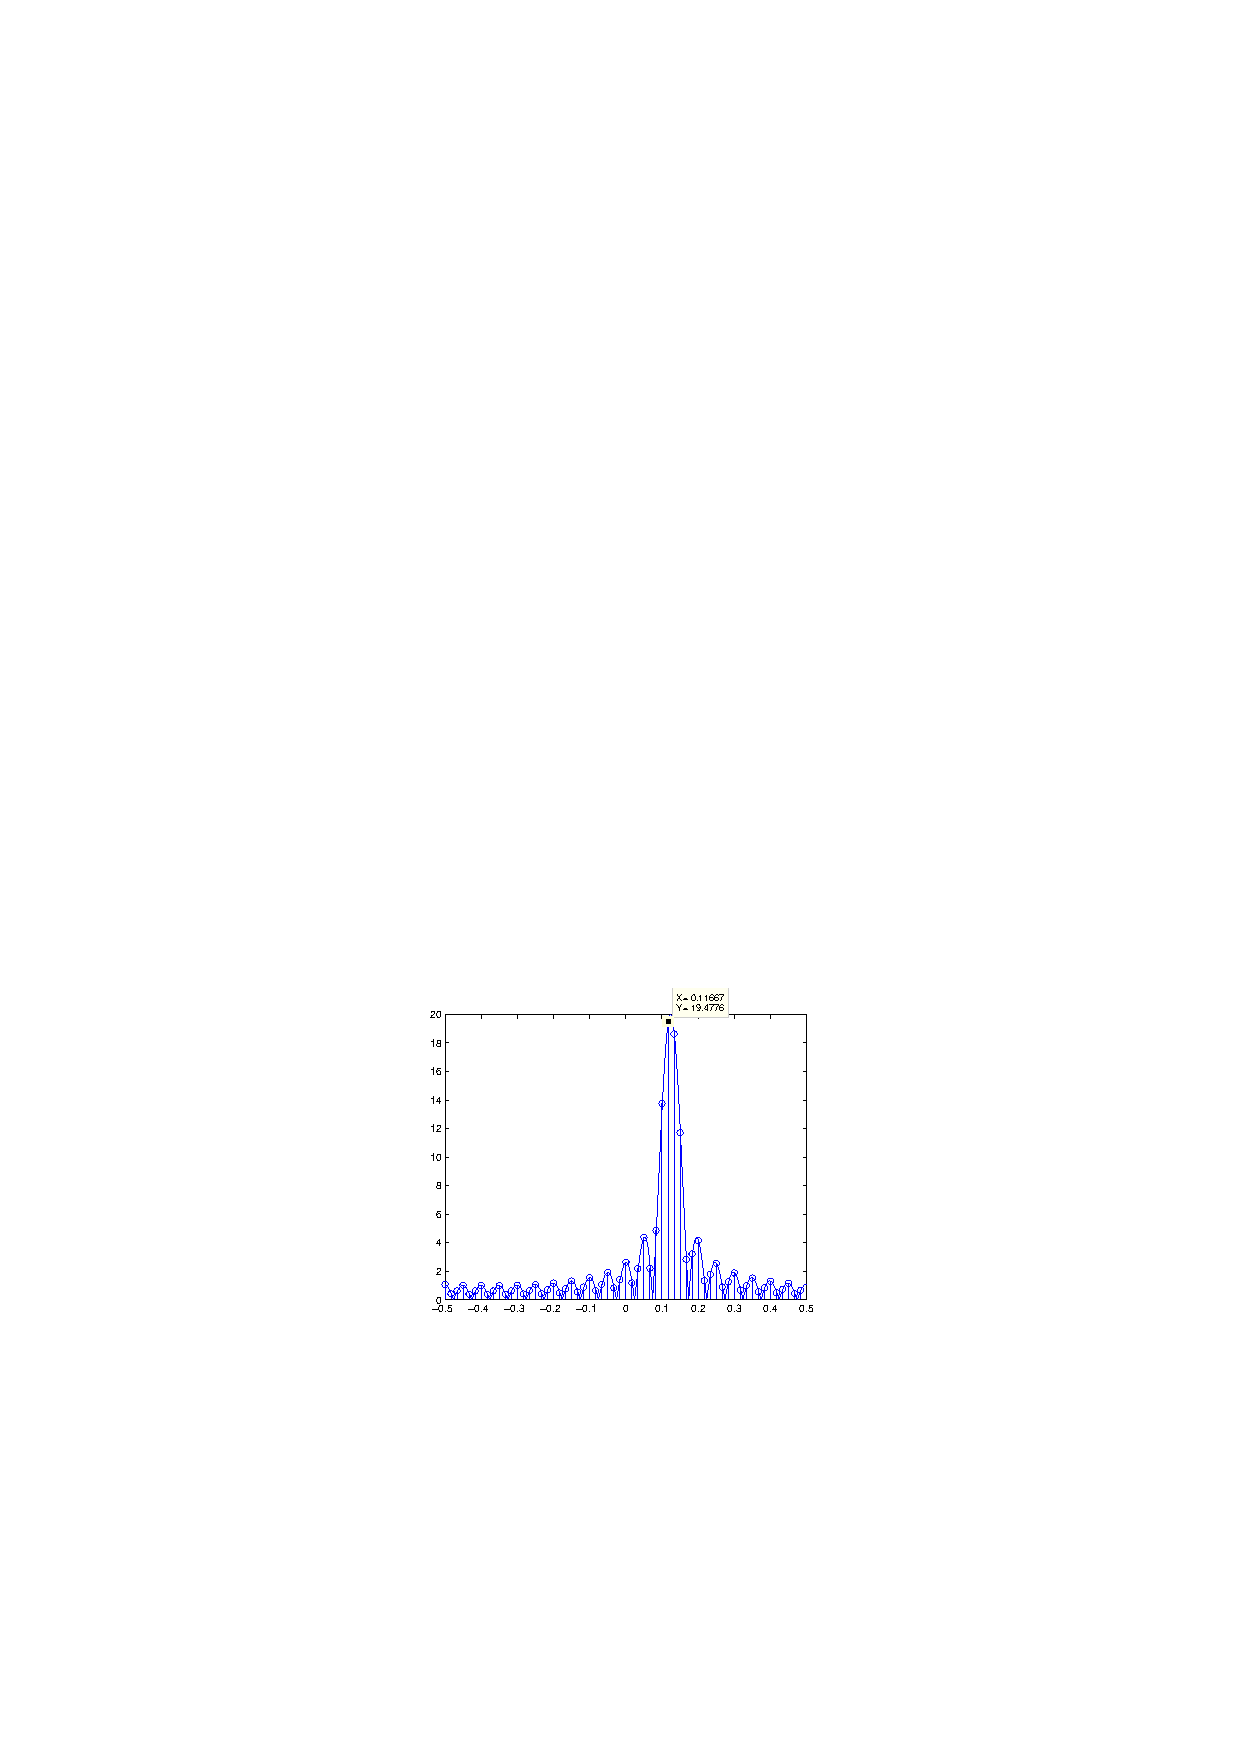
\includegraphics[width=0.6\textwidth]{Figures/Figure2-8}\\
  \caption{La TFD d'ordre 60 de l'harmonique complexe tronqu\'{e}e superpos\'{e}e \`{a} la TFtD. Le maximum de la TFD est atteint pour $k=7$, soit une fr\'{e}quence de $7/60=0$, 11667 et une erreur d'estimation de 0,0063}\label{fig:figure2-8}
\end{figure}




\subsection{S\'{e}paration de deux exponentielles complexes et fen\^{e}trage}
Cette fois-ci on poss\`{e}de un signal plus complexe qui est la somme de deux harmoniques complexes sur $\zset$
$$
u_{n}=A_{0}\rme^{2\rmi\pi\nu_{0}n}+A_{1}\rme^{2\rmi\pi\nu_{1}n}
$$
Les inconnues ici, sont les amplitudes $A_{0}$ et $A_{1}$ ainsi que les fr\'{e}quences $\nu_{0}$ et $\nu_{1}$. Encore une fois on ne se donne le droit que d'observer $N$ \'{e}chantillons, et on note $u^{T}$ la suite ainsi tronqu\'{e}e.


Les graphiques de \Cref{fig:figure2-9} \`{a} \Cref{figure:2-12} illustrent le probl\`{e}me de la r\'{e}solution fr\'{e}quentielle en calculant la TFtD de $u^{T}$ pour diff\'{e}rentes valeurs de $N$.

On constate qu'il faut au moins avoir $|\nu_{0}-\nu_{1}|>1/N$ pour pouvoir distinguer deux pics sur la TFtD. Sinon, les deux pics se confondent en un seul et il sera impossible de distinguer $\nu_{0}$ et $\nu_{1}.$

\begin{figure}
  \centering
  % Requires \usepackage{graphicx}
  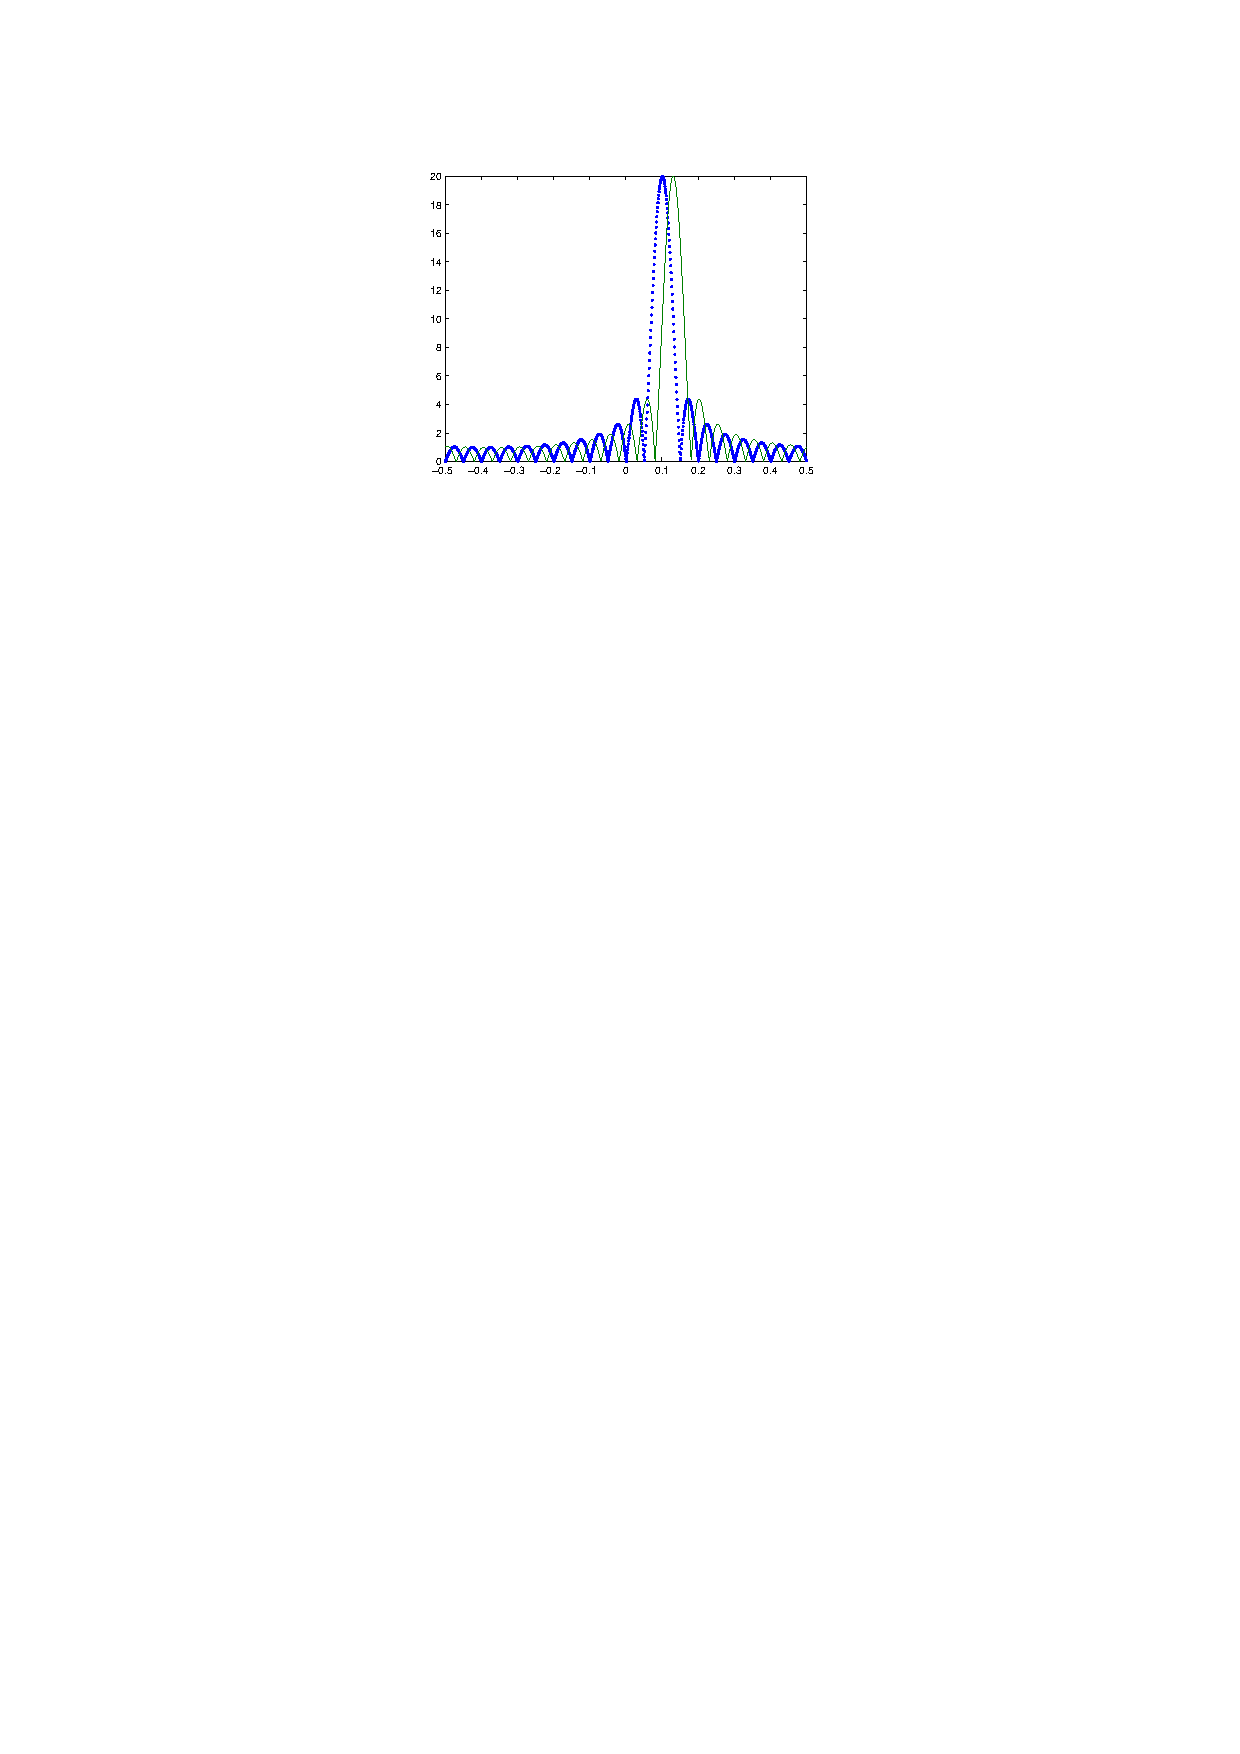
\includegraphics[width=0.6\textwidth]{Figures/Figure2-9}\\
  \caption{On a utilis\'{e} seulement $N=20$ \'{e}chantillons pour tracer la TFtD de deux ondes (l'une en pointill\'{e}s, l'autre en trait plein) de m\^{e}me module et de fr\'{e}quences 0,1 et 0,13.}\label{fig:figure2-9}
\end{figure}

\begin{figure}
  \centering
  % Requires \usepackage{graphicx}
  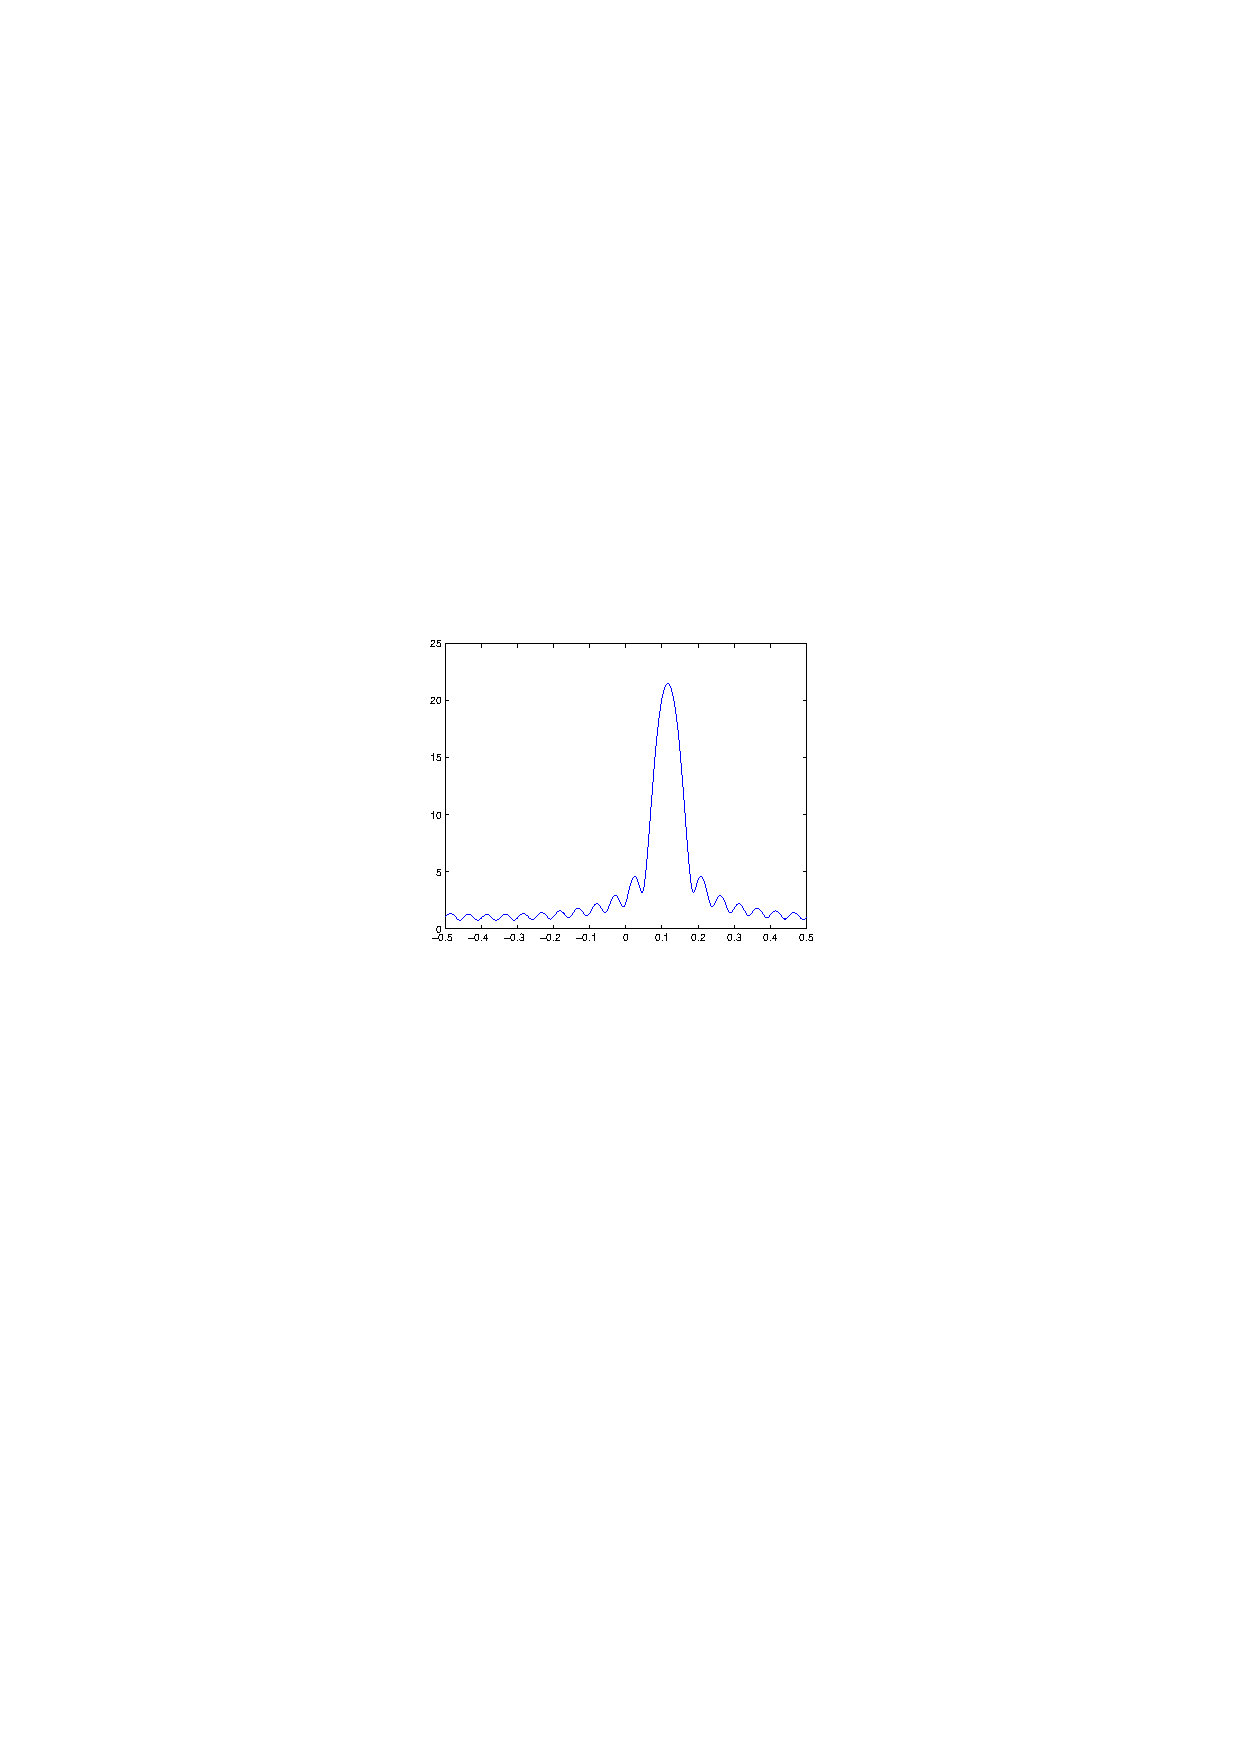
\includegraphics[width=0.6\textwidth]{Figures/Figure2-10}\\
  \caption{TFtD de la somme des deux ondes tronqu\'{e}es \`{a} 30 \'{e}chantillons (figure 2.9). On ne peut pas distinguer la superposition des deux harmoniques complexes dans le signal.}\label{fig:figure2-10}
\end{figure}

\begin{figure}
  \centering
  % Requires \usepackage{graphicx}
  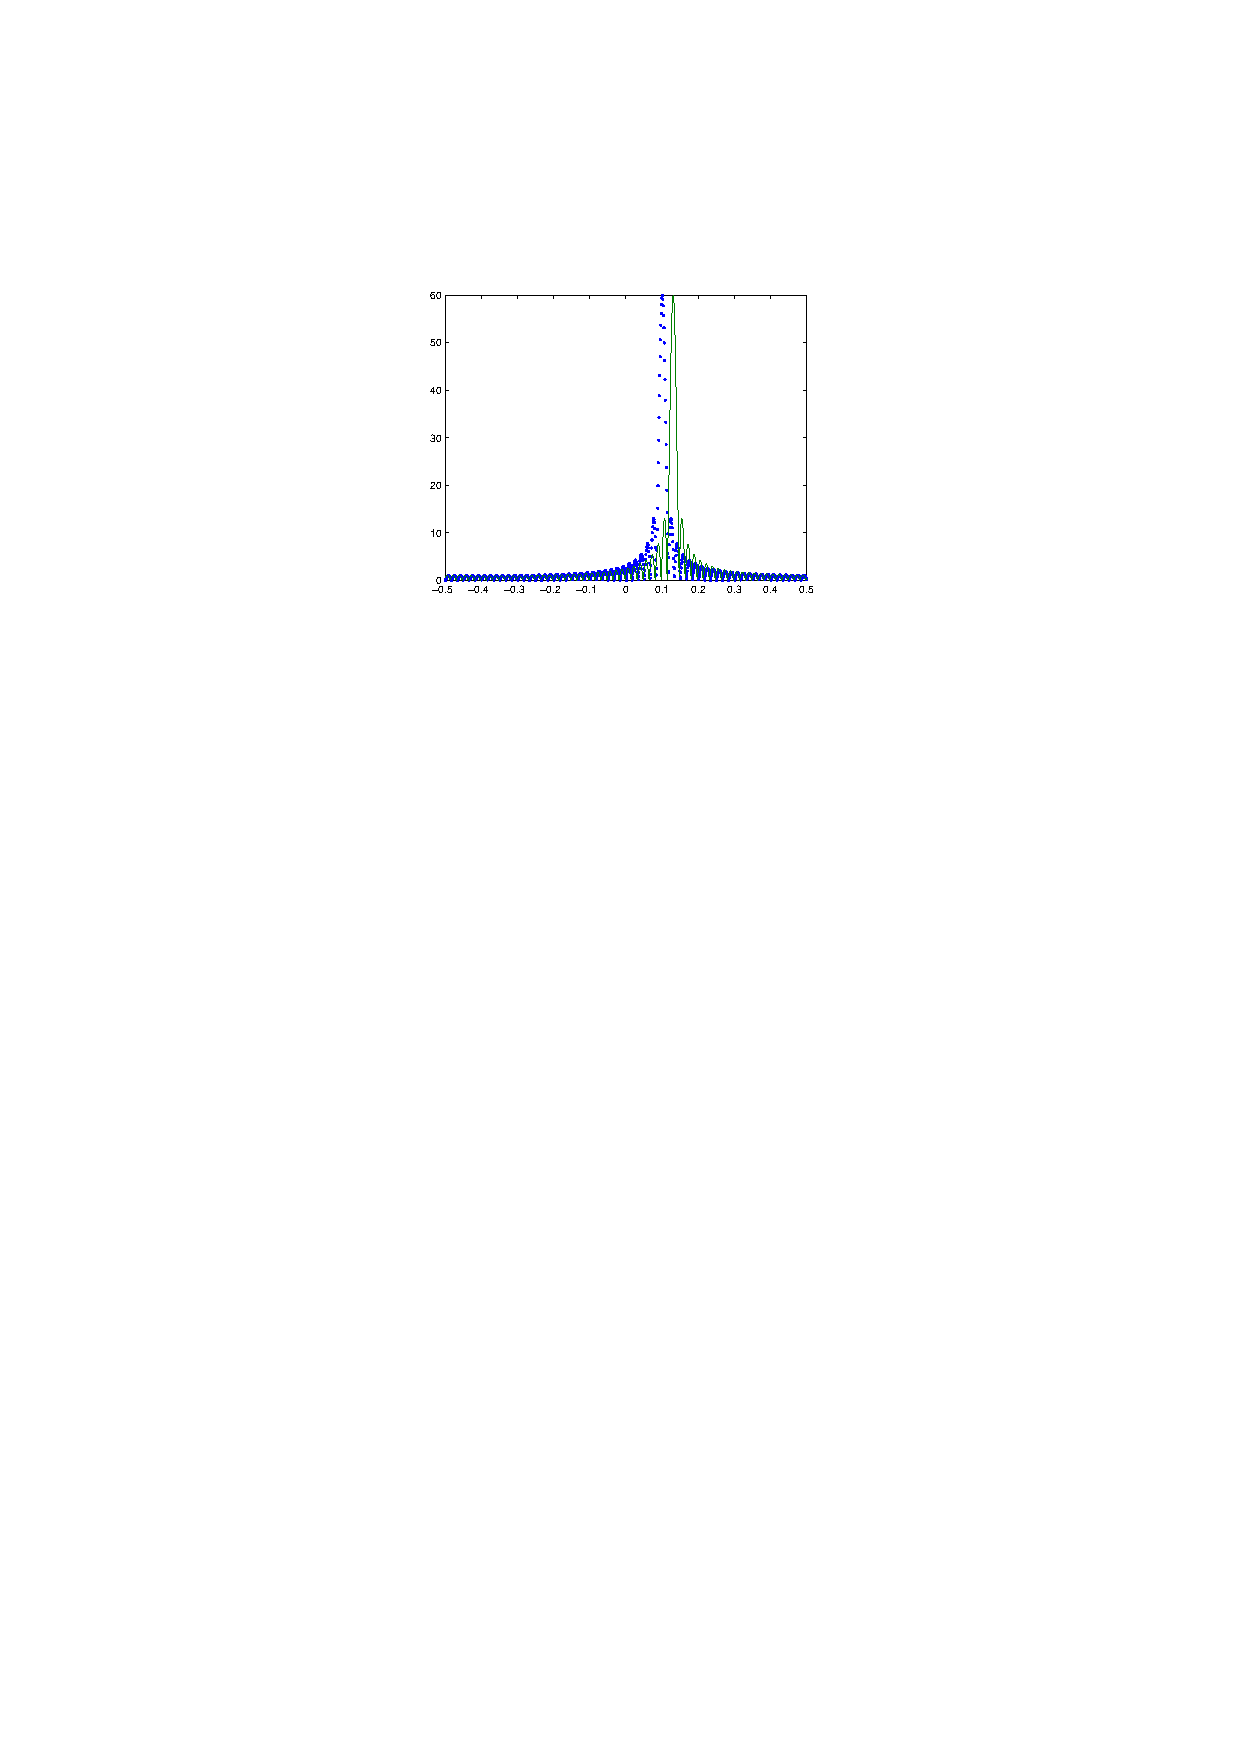
\includegraphics[width=0.6\textwidth]{Figures/Figure2-11}\\
  \caption{On a utilis\'{e} seulement $N=20$ \'{e}chantillons pour tracer la TFtD de deux ondes (l'une en pointill\'{e}s, l'autre en trait plein) de m\^{e}me module et de fr\'{e}quences 0,1 et 0,13.}\label{fig:figure2-11}
\end{figure}


\begin{figure}
  \centering
  % Requires \usepackage{graphicx}
  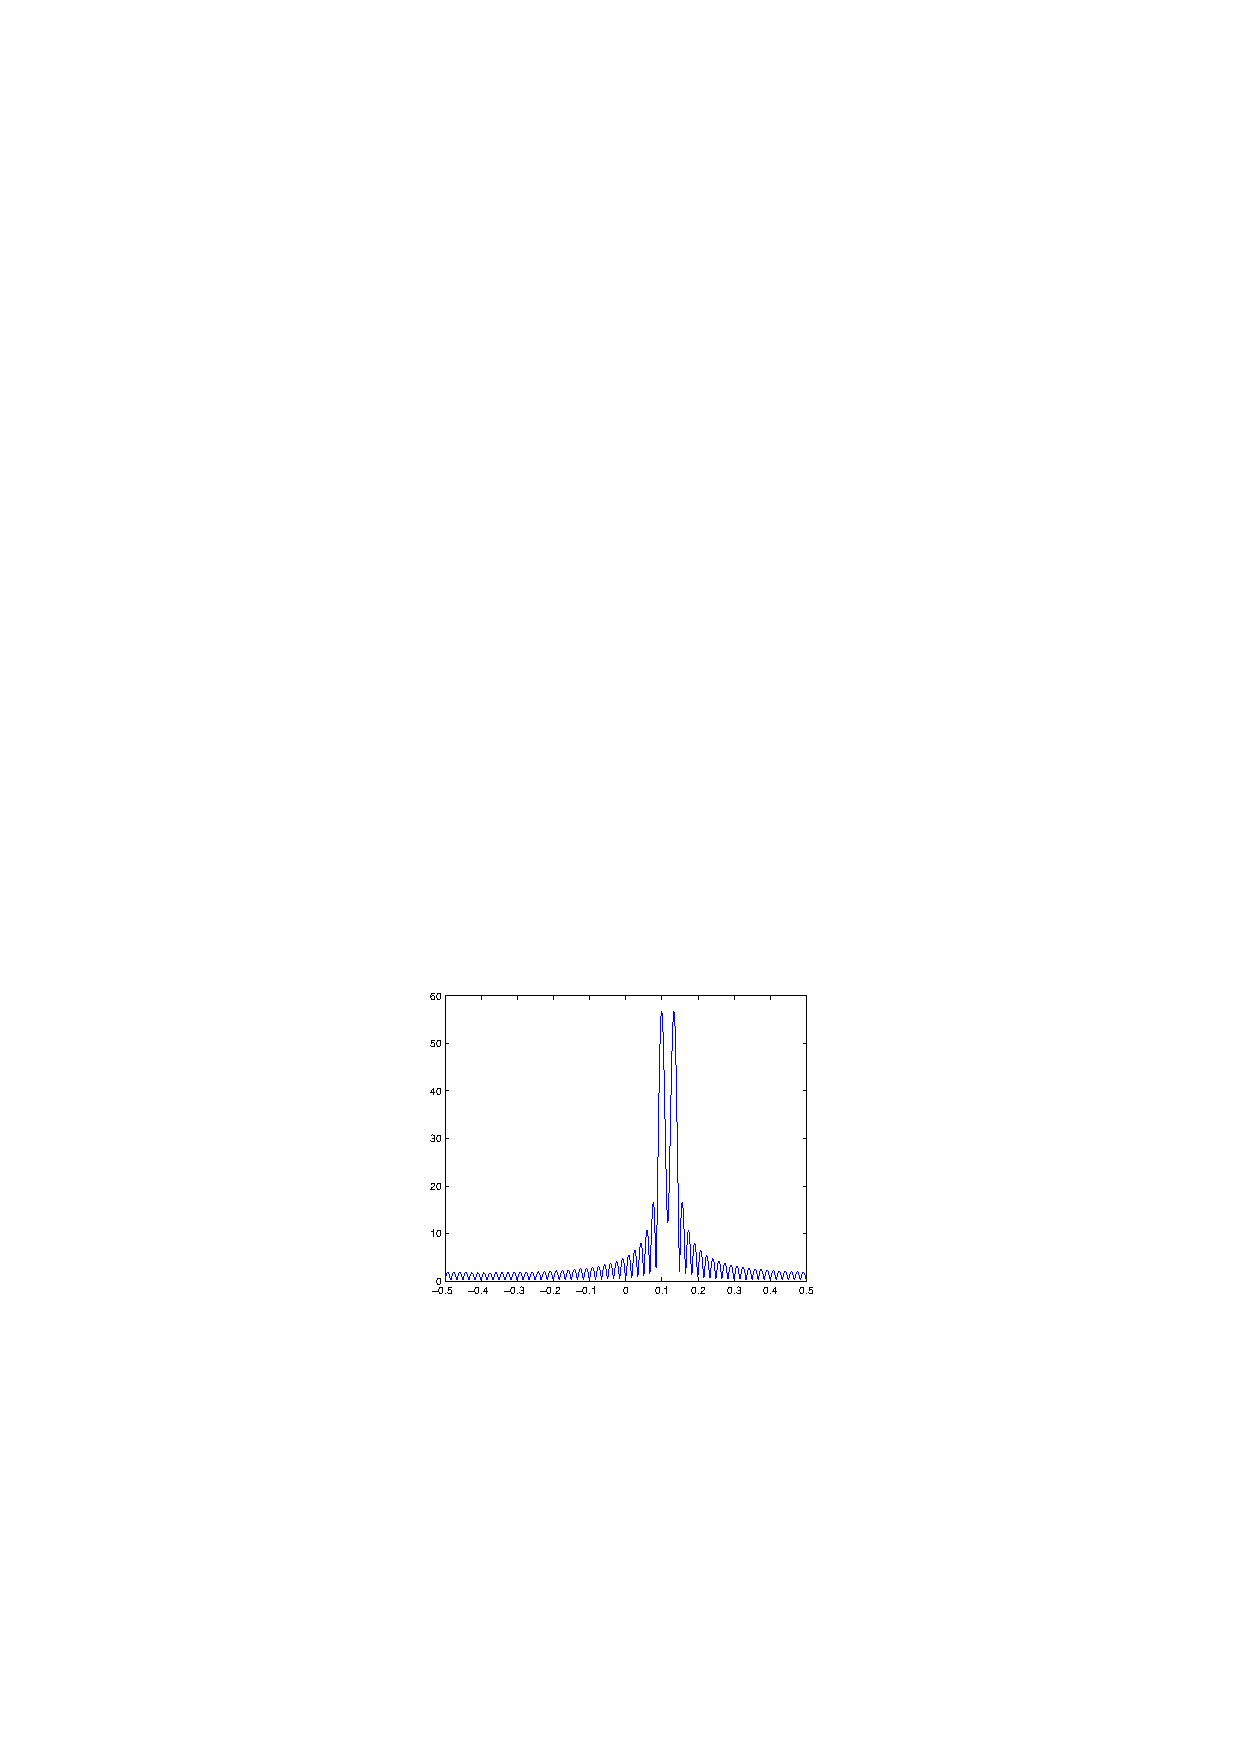
\includegraphics[width=0.6\textwidth]{Figures/Figure2-12}\\
  \caption{TFtD de la somme des deux ondes tronqu\'{e}es \`{a} 60 \'{e}chantillons (figure 2.11). Cette fois on distingue bien les deux ondes. Il a fallu prendre un nombre d'\'{e}chantillons $N$ sup\'{e}rieur \`{a} $1/(0.13-0.1)=33.3$ pour arriver \`{a} distinguer les deux.}\label{fig:figure2-12}
\end{figure}


\begin{figure}
  \centering
  % Requires \usepackage{graphicx}
  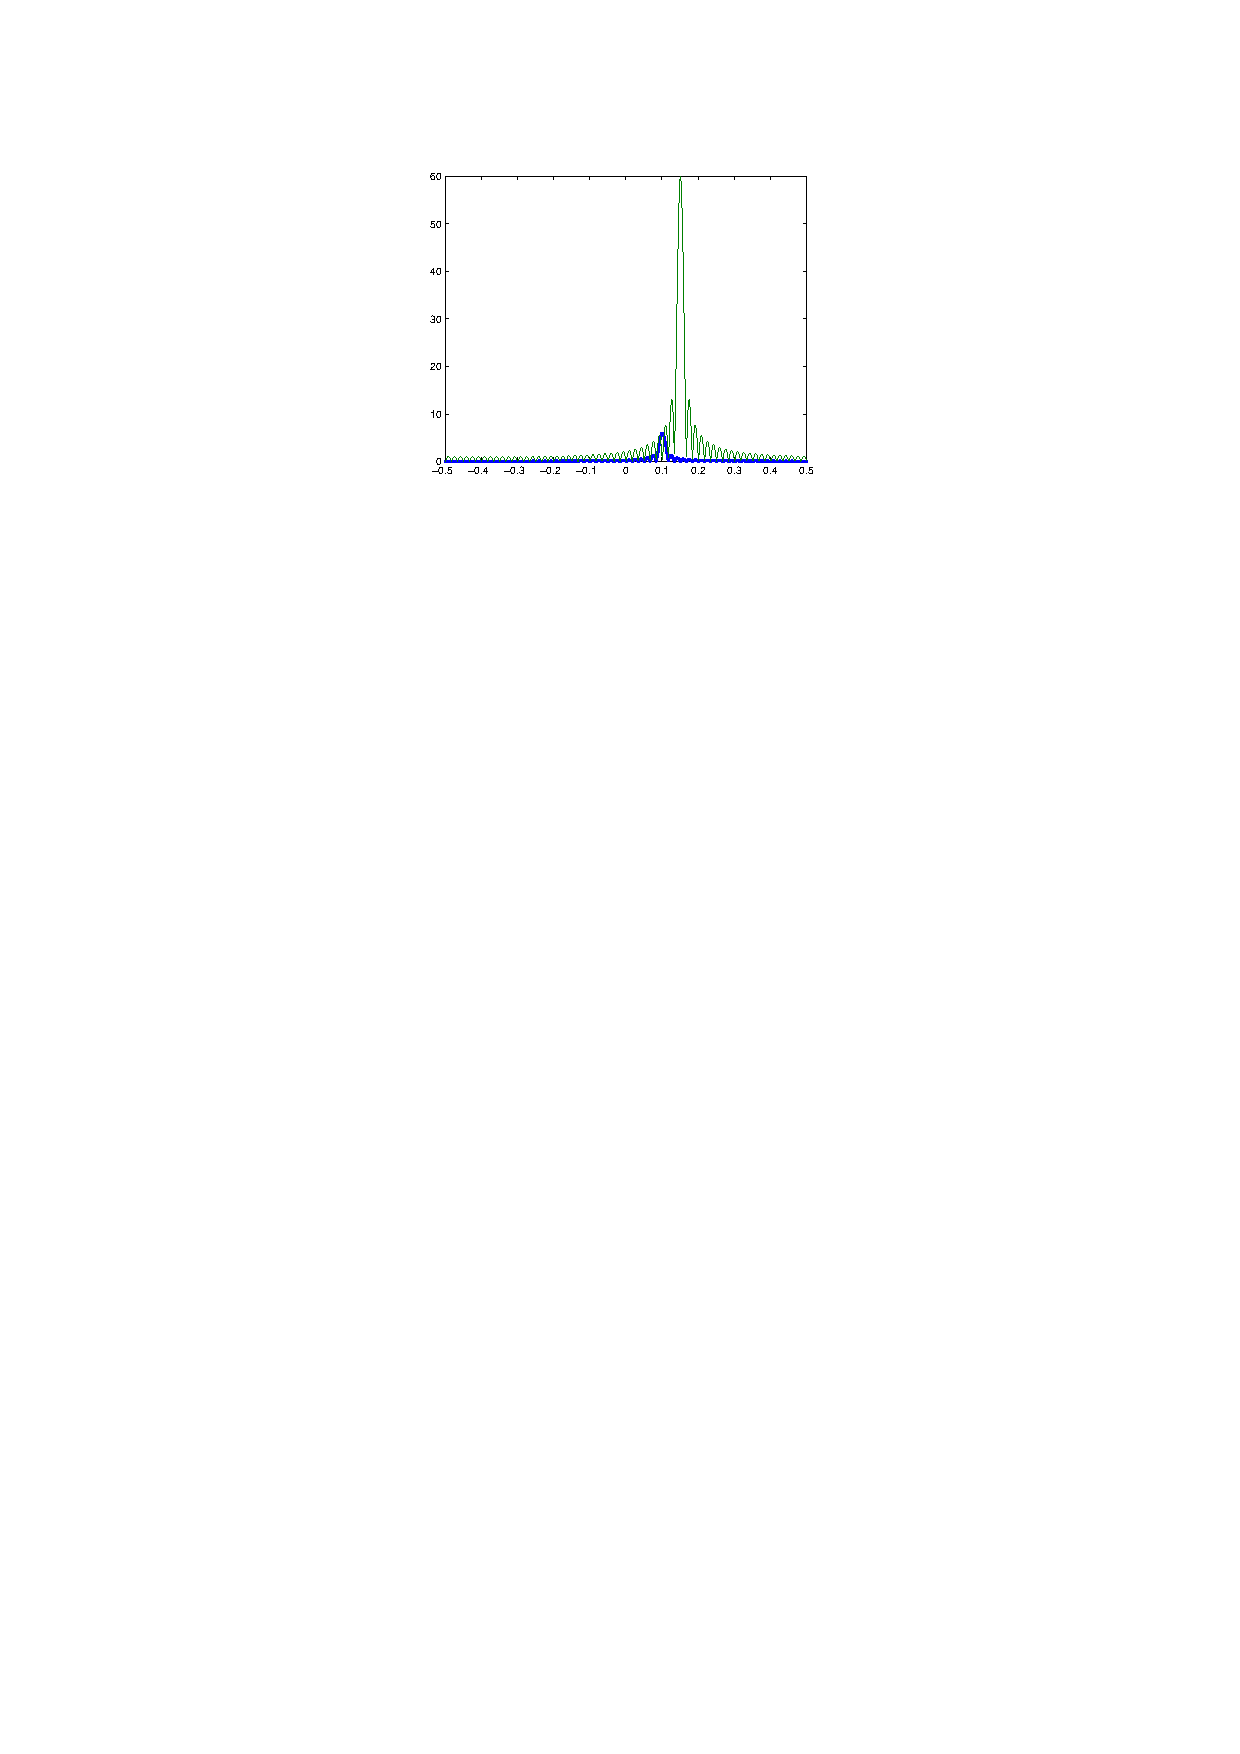
\includegraphics[width=0.6\textwidth]{Figures/Figure2-13}\\
  \caption{TFtD de deux ondes tronqu\'{e}es dont l'une a une amplitude 10 fois plus petite que l'autre. La plus petite des deux est cach\'{e}e par les lobes secondaires de la TFtD de l'autre.}\label{fig:figure2-13}
\end{figure}


\begin{figure}
  \centering
  % Requires \usepackage{graphicx}
  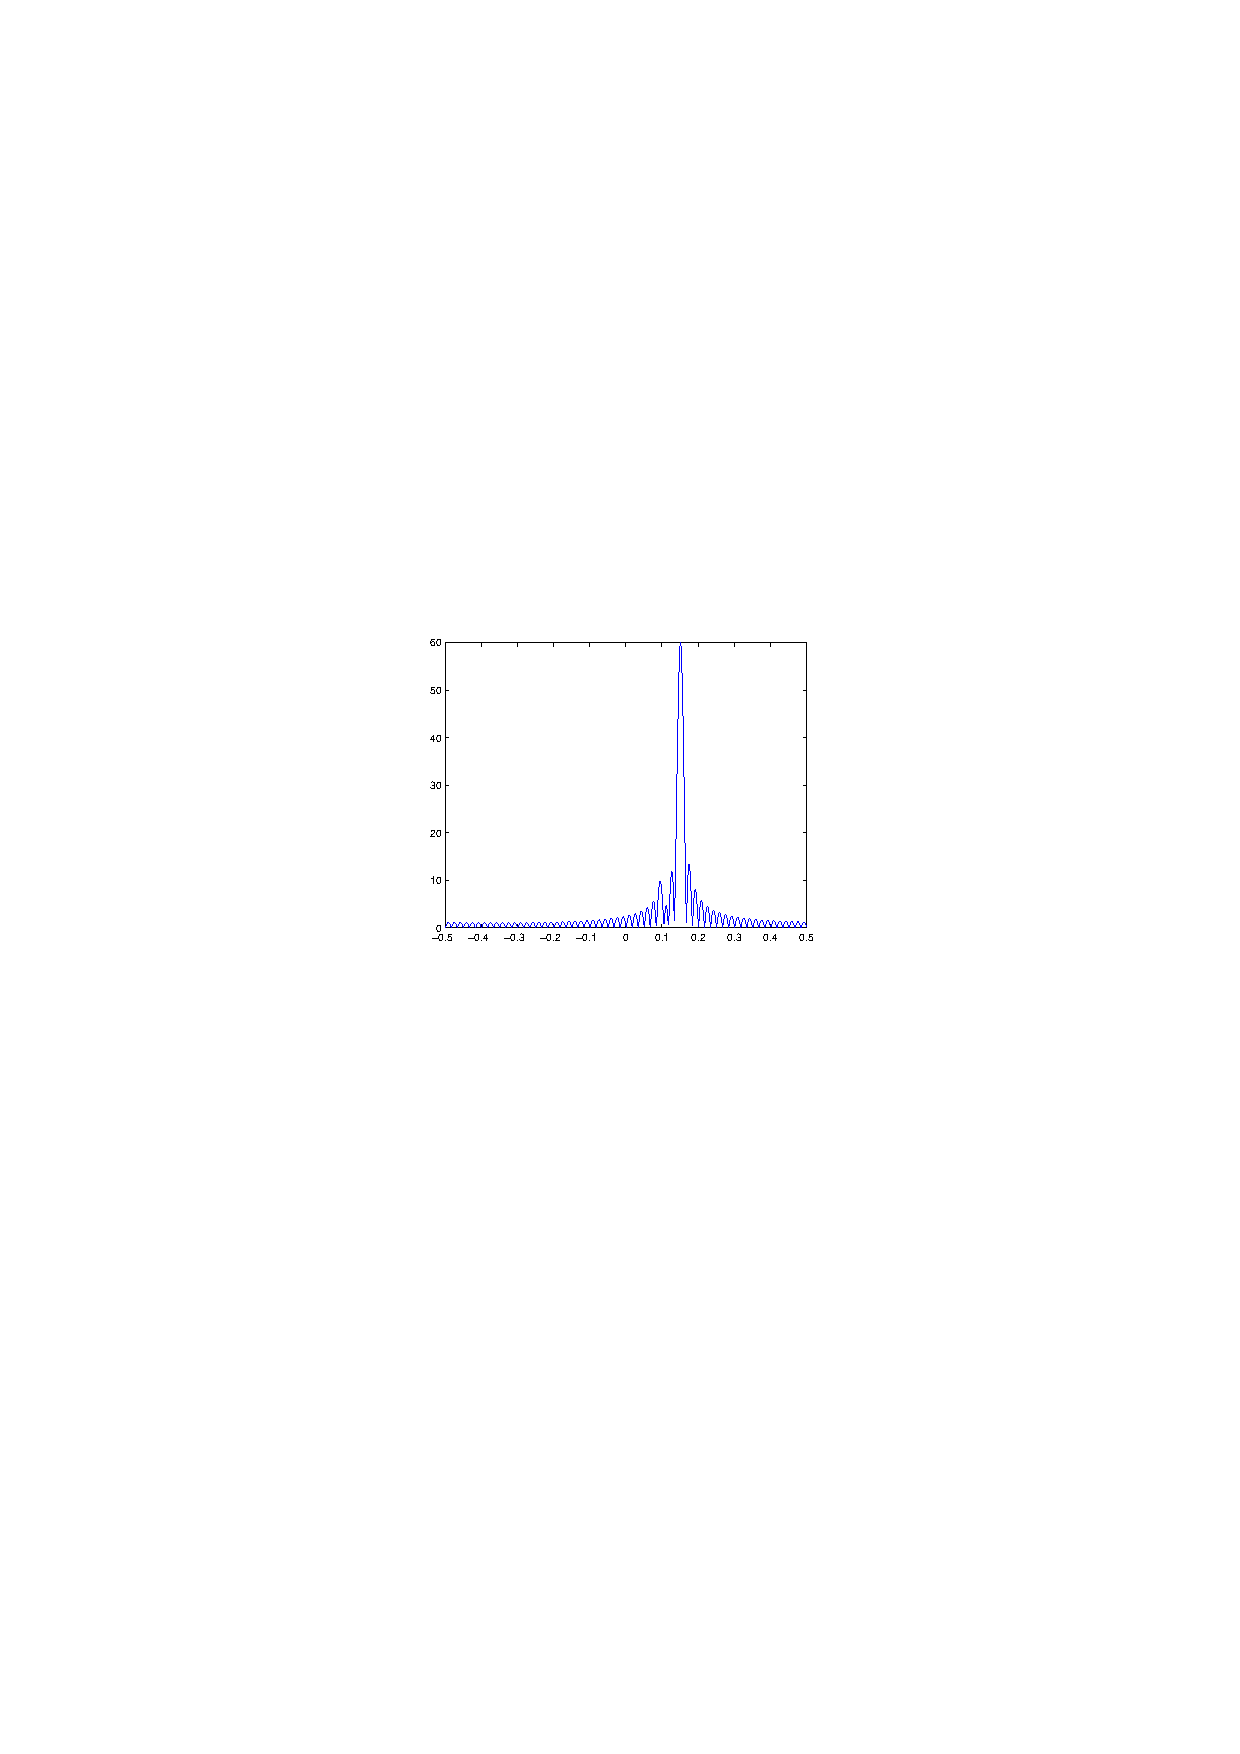
\includegraphics[width=0.6\textwidth]{Figures/Figure2-14}\\
  \caption{TFtD de la somme des deux ondes tronqu\'{e}es. Il est difficile de d\'{e}celer la pr\'{e}sence de l'harmonique complexe de faible amplitude.}\label{fig:figure2-14}
\end{figure}

On dit que $1/N$ est la r\'{e}solution fr\'{e}quentielle. Il faut augmenter $N$ pour pouvoir s\'{e}parer des fr\'{e}quences proches l'une de l'autre.


Les graphiques \Cref{fig:figure2-13} et \Cref{fig:figure2-13} montrent une situation o\`{u} $A_{1}$ est beaucoup plus grand que $A_{0}$. On constate que les lobes secondaires de la TFtD de l'harmonique complexe (tronqu\'{e}e) $\nu_{1}$ cachent jusqu'au lobe principal de l'harmonique complexe tronqu\'{e}e de fr\'{e}quence $\nu_{0}$. Cela est du au fait que la troncature choisie est trop brutale. Pour obtenir $u^{T}$ nous avons multipli\'{e} $u$ par une fen\^{e}tre rectangulaire que l'on va noter $c$:

$c_{n}=\left\{\begin{array}{l}
1\ \mathrm{s}\mathrm{i}\ 0\leq n<N\\
0\ \mathrm{s}\mathrm{i}\mathrm{n}\mathrm{o}\mathrm{n}
\end{array}\right.$
et on a fait $u^{T}=u.c$. Comme vu plus haut la TFtD de $u^{T}$ est la convolution de la
TFtD de $u$ avec celle de $c$.
\begin{figure}
  \centering
  % Requires \usepackage{graphicx}
  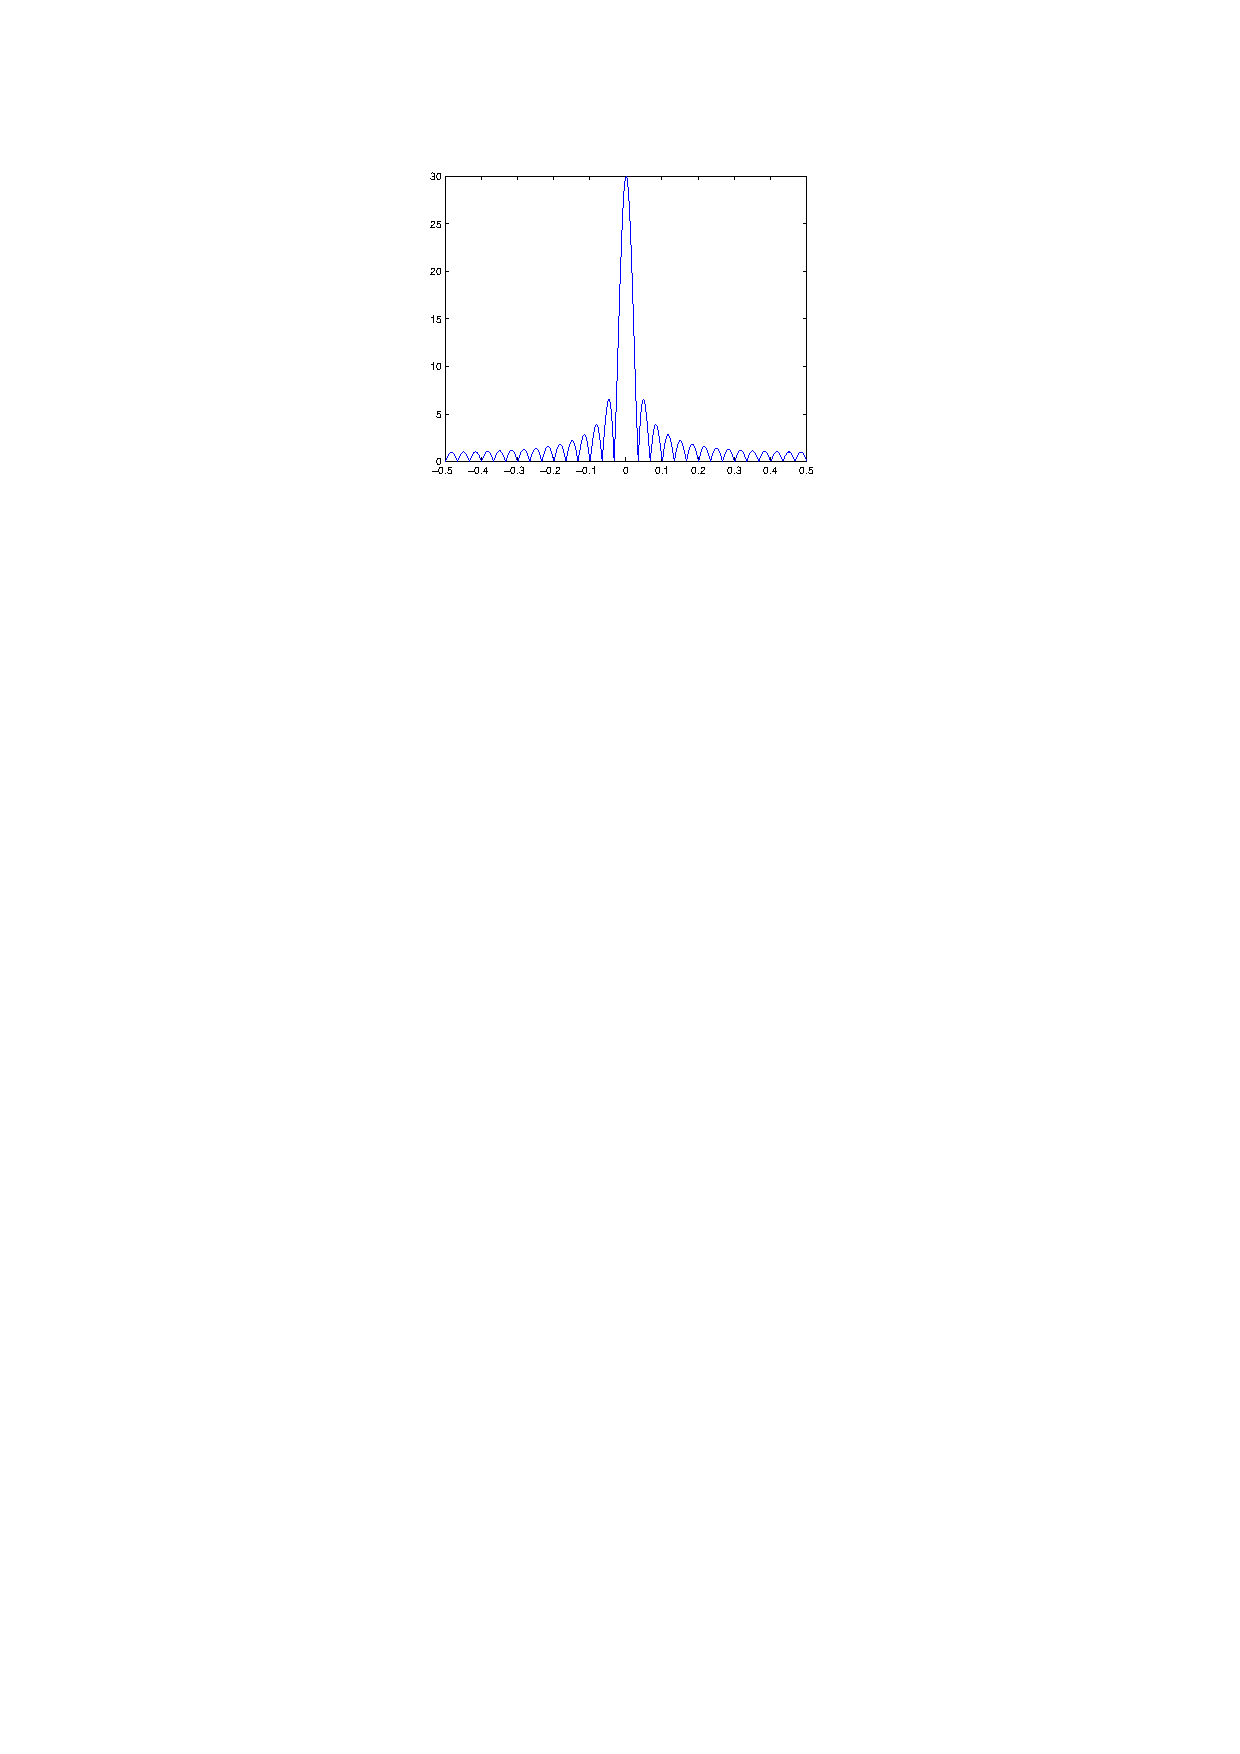
\includegraphics[width=0.6\textwidth]{Figures/Figure2-15}\\
  \caption{TFtD d'un cr\'{e}neau de taille 30.}\label{fig:figure2-15}
\end{figure}

\begin{figure}
  \centering
  % Requires \usepackage{graphicx}
  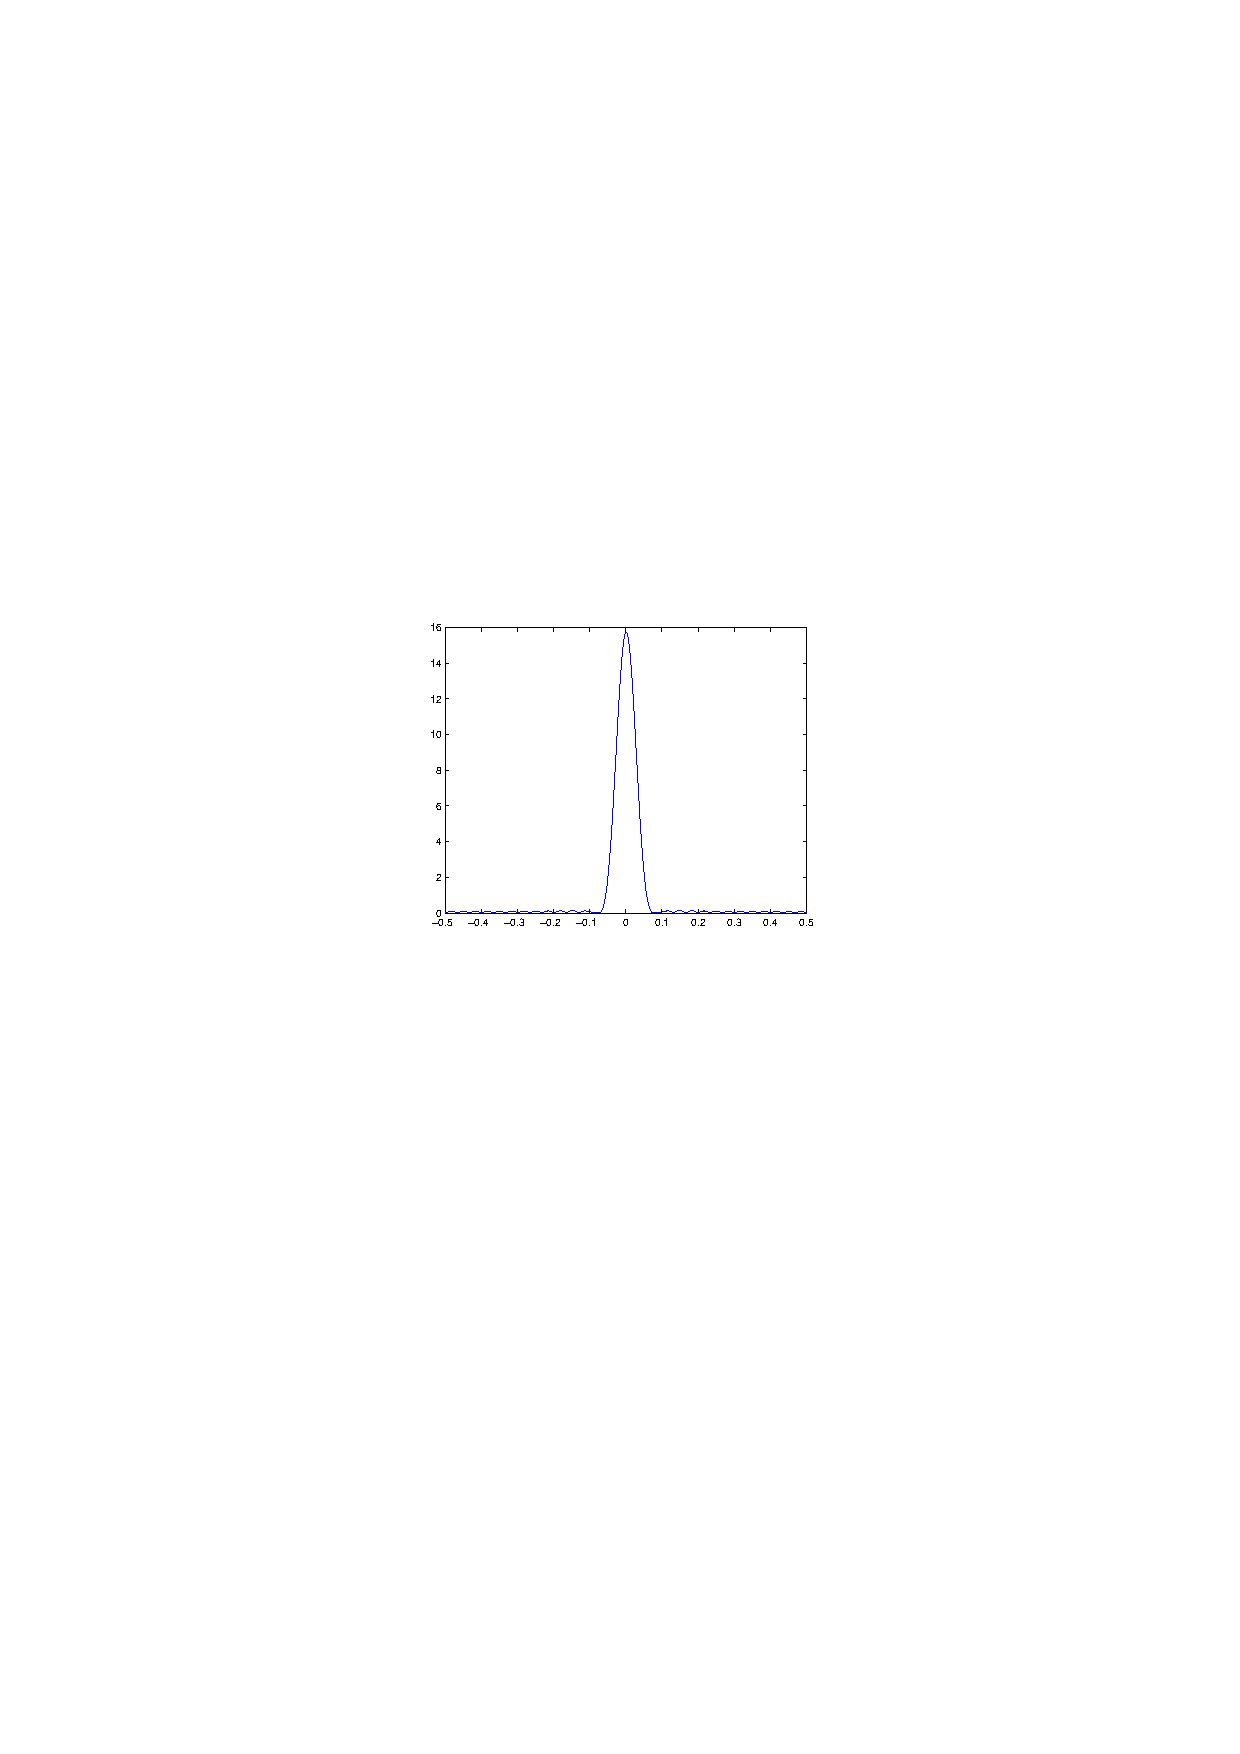
\includegraphics[width=0.6\textwidth]{Figures/Figure2-16}\\
  \caption{TFtD d'une fen\^{e}tre de Hamming de taille $N=30.$}\label{fig:figure2-16}
\end{figure}
\Cref{fig:figure2-15} montre le module de la TFtD de $c$. Si l'on trouve une fen\^{e}tre dont la TFtD pr\'{e}sente des lobes secondaires moins pro\'{e}minents on peut esp\'{e}rer r\'{e}soudre le probl\`{e}me que pose la s\'{e}paration des deux ondes de notre m\'{e}lange. Une fen\^{e}tre propos\'{e}e est la fen\^{e}tre de Hamming d\'{e}finit par

$h_{n}=\left\{\begin{array}{l}
0.\ 54-0.46cos(2\pi\frac{n}{N-1})\ \mathrm{s}\mathrm{i}\ 0\leq n<N\\
0\ \mathrm{s}\mathrm{i}\mathrm{n}\mathrm{o}\mathrm{n}
\end{array}\right.$

\Cref{fig:figure2-16} montre la TFtD de la fen\^{e}tre de Hamming. 
Par rapport \`{a} celle de $c$ (cr\'{e}neau), on constate deux choses
\begin{enumerate}
\item Le lobe central est plus \'{e}tal\'{e} : ceci implique une perte de r\'{e}solution fr\'{e}quentielle. On passe d'une r\'{e}solution de l'ordre de $1/N$ \`{a} une r\'{e}solution de l'ordre de $2/N.$
\item Les lobes secondaires sont très atténués par rapport au  lobe central, ce qui permet de distinguer deux ondes dont les amplitudes diff\`{e}rent grandement.
\end{enumerate}
\Cref{fig:figure2-17}et \Cref{fig:figure2-18}  montrent comment la multiplication par une fen\^{e}tre de Hamming plut\^{o}t qu'une troncature brutale permet de distinguer une onde de faible amplitude.


\begin{figure}
  \centering
  % Requires \usepackage{graphicx}
  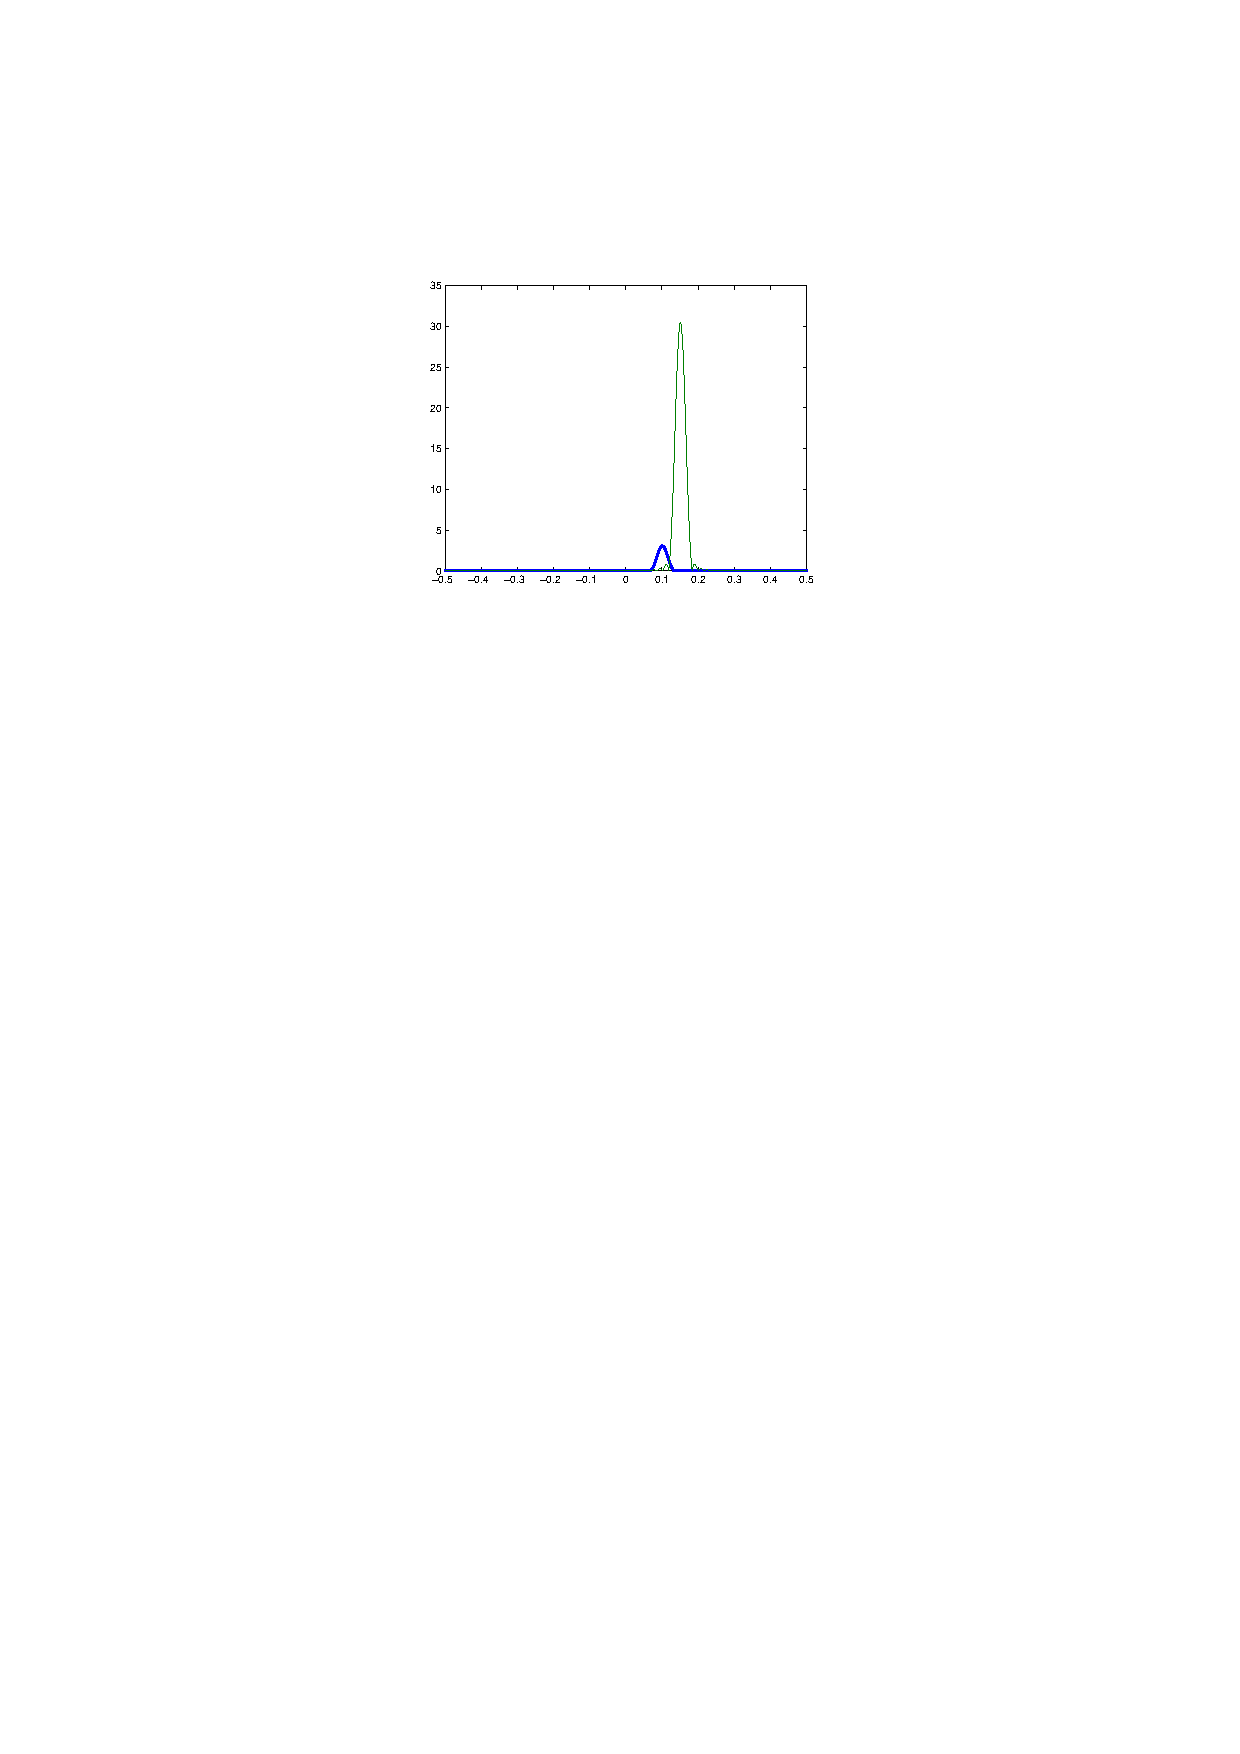
\includegraphics[width=0.6\textwidth]{Figures/Figure2-17}\\
  \caption{M\^{e}me figure que \Cref{fig:figure2-13} mais en ayant multipli\'{e} le signal par une fen\^{e}tre de Hamming. Cette fois l'harmonique complexe de faible amplitude est bien au dessus des lobes secondaires de l'harmonique complexe de forte amplitude.}\label{fig:figure2-17}
\end{figure}


\begin{figure}
  \centering
  % Requires \usepackage{graphicx}
  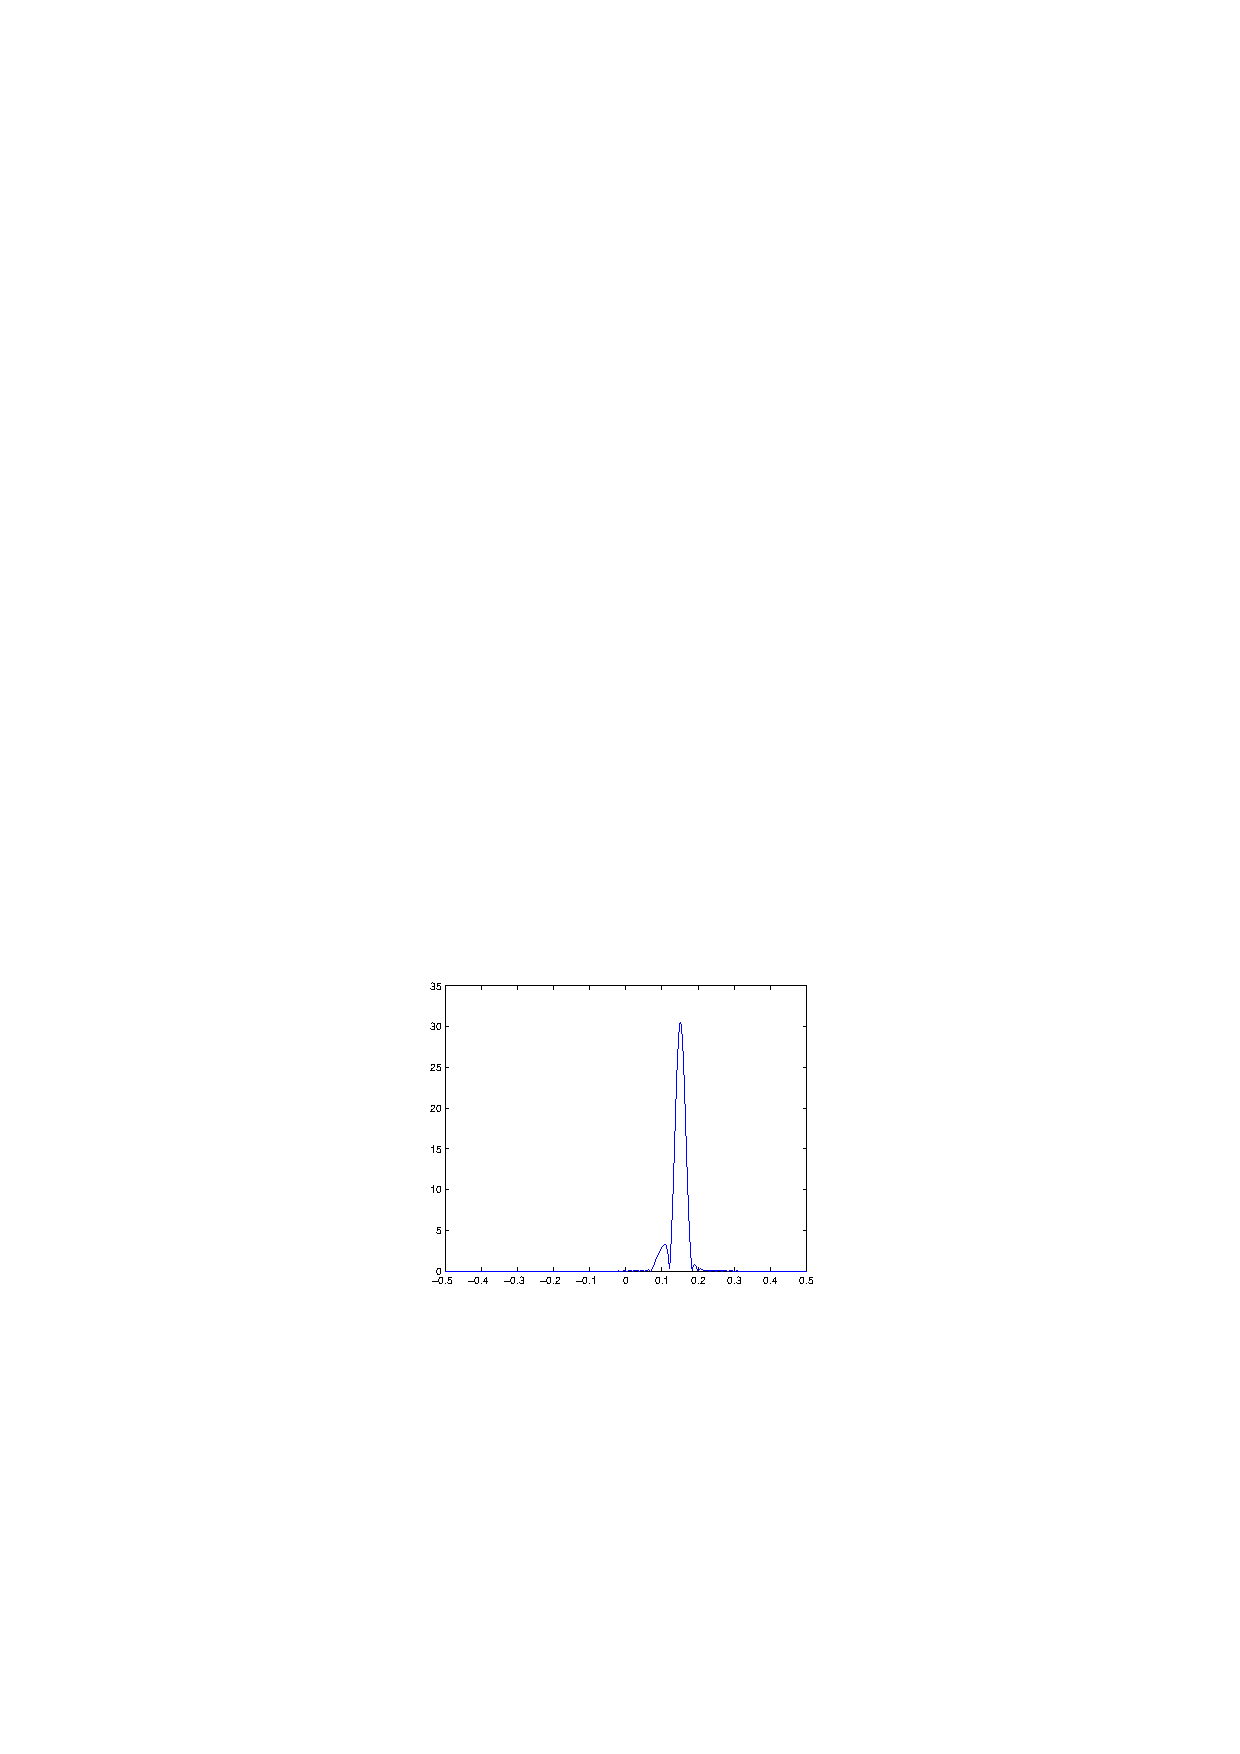
\includegraphics[width=0.6\textwidth]{Figures/Figure2-18}\\
  \caption{M\^{e}me figure que \Cref{fig:figure2-14} mais en ayant multipli\'{e} le signal contre une fen\^{e}tre de hamming plut\^{o}t que de la tronquer brutalement. Cette fois-ci on constate bien un deuxi\`{e}me lobe qui ne peut \^{e}tre confondu avec le lobe secondaire engendr\'{e} par l'harmonique complexe pr\'{e}dominante, car ces lobes secondaires sont bien plus faibles d'apr\`{e}s \Cref{fig:figure2-16}}\label{fig:figure2-18}
\end{figure}


\section{Transformée de Fourier à Court Terme (TFCT)}
La Transform\'{e}e de Fourier \`{a} Court Terme (TFCT) n'est pas \`{a} proprement parler une transformation de Fourier. Elle n'en a pas les propri\'{e}t\'{e}s alg\'{e}briques remarquables, c'est pourtant un outil essentiel en traitement du signal. Cet outil est bas\'{e} sur la constatation d\'{e}j\`{a} faite plus haut que le contenu fr\'{e}quentiel d'un signal peut \'{e}voluer au cours du temps. Elle se d\'{e}finit naivement comme une analyse locale des composantes fr\'{e}quentielles du si- gnal. Plus pr\'{e}cis\'{e}ment, pour chaque instant $n$, on extrait un certain nombre d'\'{e}chantillons du signal \'{e}tudi\'{e} autour du point $n$ que l'on \'{e}tudie par les moyens $\mathrm{v}\mathrm{u}\mathrm{s}$ ci-dessus (fen\^{e}trage et TFD d'ordres arbitraires).

Si $u$ est une suite d\'{e}finie sur $\zset$. On fixe une fen\^{e}tre} $w_{0}, \ldots, w_{n}$ de taille
$N$ et on choisit un entier $M\geq N.$ La Transform\'{e}e de Fourier \`{a} Court Terme de $u$ de
fen\^{e}tre} $w$ et de pr\'{e}cision} $1/M$ est une fonction, que l'on note $U$ d\'{e}finie sur $\displaystyle \zset\times\frac{\{0,\ldots,M-1\}}{M}$par
$$
\forall(n,\ k)\in \zset\times\{0,\ \ldots,\ M-1\},\ U(n,\ \frac{k}{M})=\sum_{m\in \zset}u_{m}w_{n-m}\rme^{-2\rmi\pi \frac{k}{M}m}
$$
On peut aussi consid\'{e}rer} $U$ comme une fonction d\'{e}finie sur} $\displaystyle \mathrm{z}\times[-\frac{1}{2}, \displaystyle \frac{1}{2}$ [que l'on \'{e}chantiollonnera aussi finement que l'on veut suivant la seconde variable en augmentant la valeur de $M$
(ordre de la} $TFD$)
$$
\forall(n,\ \nu)\in \zset\times[-\frac{1}{2},\ \frac{1}{2}\ [,\ U(n,\ \nu)=\sum_{m\in \zset}u_{m}w_{m-n}\rme^{-2\rmi\pi  1/m}
$$
On distingue cette notation de la notation} $U$ pour la} $TFD$ par le fait qu}'elle poss\`{e}de},
ici, deux variables.

\paragraph{Pour $n$ fix\'{e}}: On remarque que pour un entier $n$ fix\'{e}, la fonction $\nu\mapsto U(n,\ \nu)$ est la TFtD de la suite $l\mapsto u_{l}w_{l-n}$, c'est \`{a} dire la suite $u$ multipli\'{e}e par la $n$-translat\'{e}e de la fen\^{e}tre $w$. Il s'agit bien de ce que nous avions annonc\'{e}, autour de chaque instant $n$, on extrait une fenêtre de signal dont on calcule la TFtD (à l'aide d'une TFD dont le nombre de coefficients peut être choisi de façon arbitraire).

\paragraph{Pour $\nu$ fix\'{e}}: Pour une fr\'{e}quence $\nu$ fix\'{e}e avec $n$ variable, on a :
$$
U(n,\ \nu)=\sum_{m\in \zset}u_{m}w_{m-n}\rme^{-2\rmi\pi  1/m}=\rme^{-2\rmi\pi  1/n}\sum_{m}u_{m}\gamma_{n-m}
$$
o\`{u} $\gamma$ est la suite d\'{e}finie par
$$
\gamma_{l}=w_{-l} \rme^{2 \rmi\pi \nu l}
$$
Le module de $U$ est alors
$$
|U(n,\ \nu)|=|(u*\gamma)_{n}|
$$
Ainsi le module de $U$ est celui de la convolution de la sym\'{e}trique de $w$ multipli\'{e}e par une harmonique complexe  de fr\'{e}quence $\nu$. Cela signifie qu'\`{a} $\nu$ fix\'{e}, le module de $U$ refl\`{e}te \`{a} quel point la fr\'{e}quence $\nu$ est pr\'{e}sente dans le signal autour du point $n$. En effet, la TFtD de $\gamma$ est centr\'{e}e autour de la fr\'{e}quence $\nu$ (la fen\^{e}tre $w$, si c'est une fen\^{e}tre de Hamming par exemple, a son spectre centr\'{e} en z\'{e}ro).


Le spectrogramme est le module au carr\'{e} de la TFCT $((n,\ \nu)\mapsto|U(n,\ \nu)|^{2})$ . On le visualise comme une image, les deux axes sont ceux des variables $n$ et $\nu$, on repr\'{e}sente la valeur du spectrogramme soit en gris, suivant la valeur (sombre pour grand et clair pour faible). 

\begin{figure}
  \centering
  % Requires \usepackage{graphicx}
  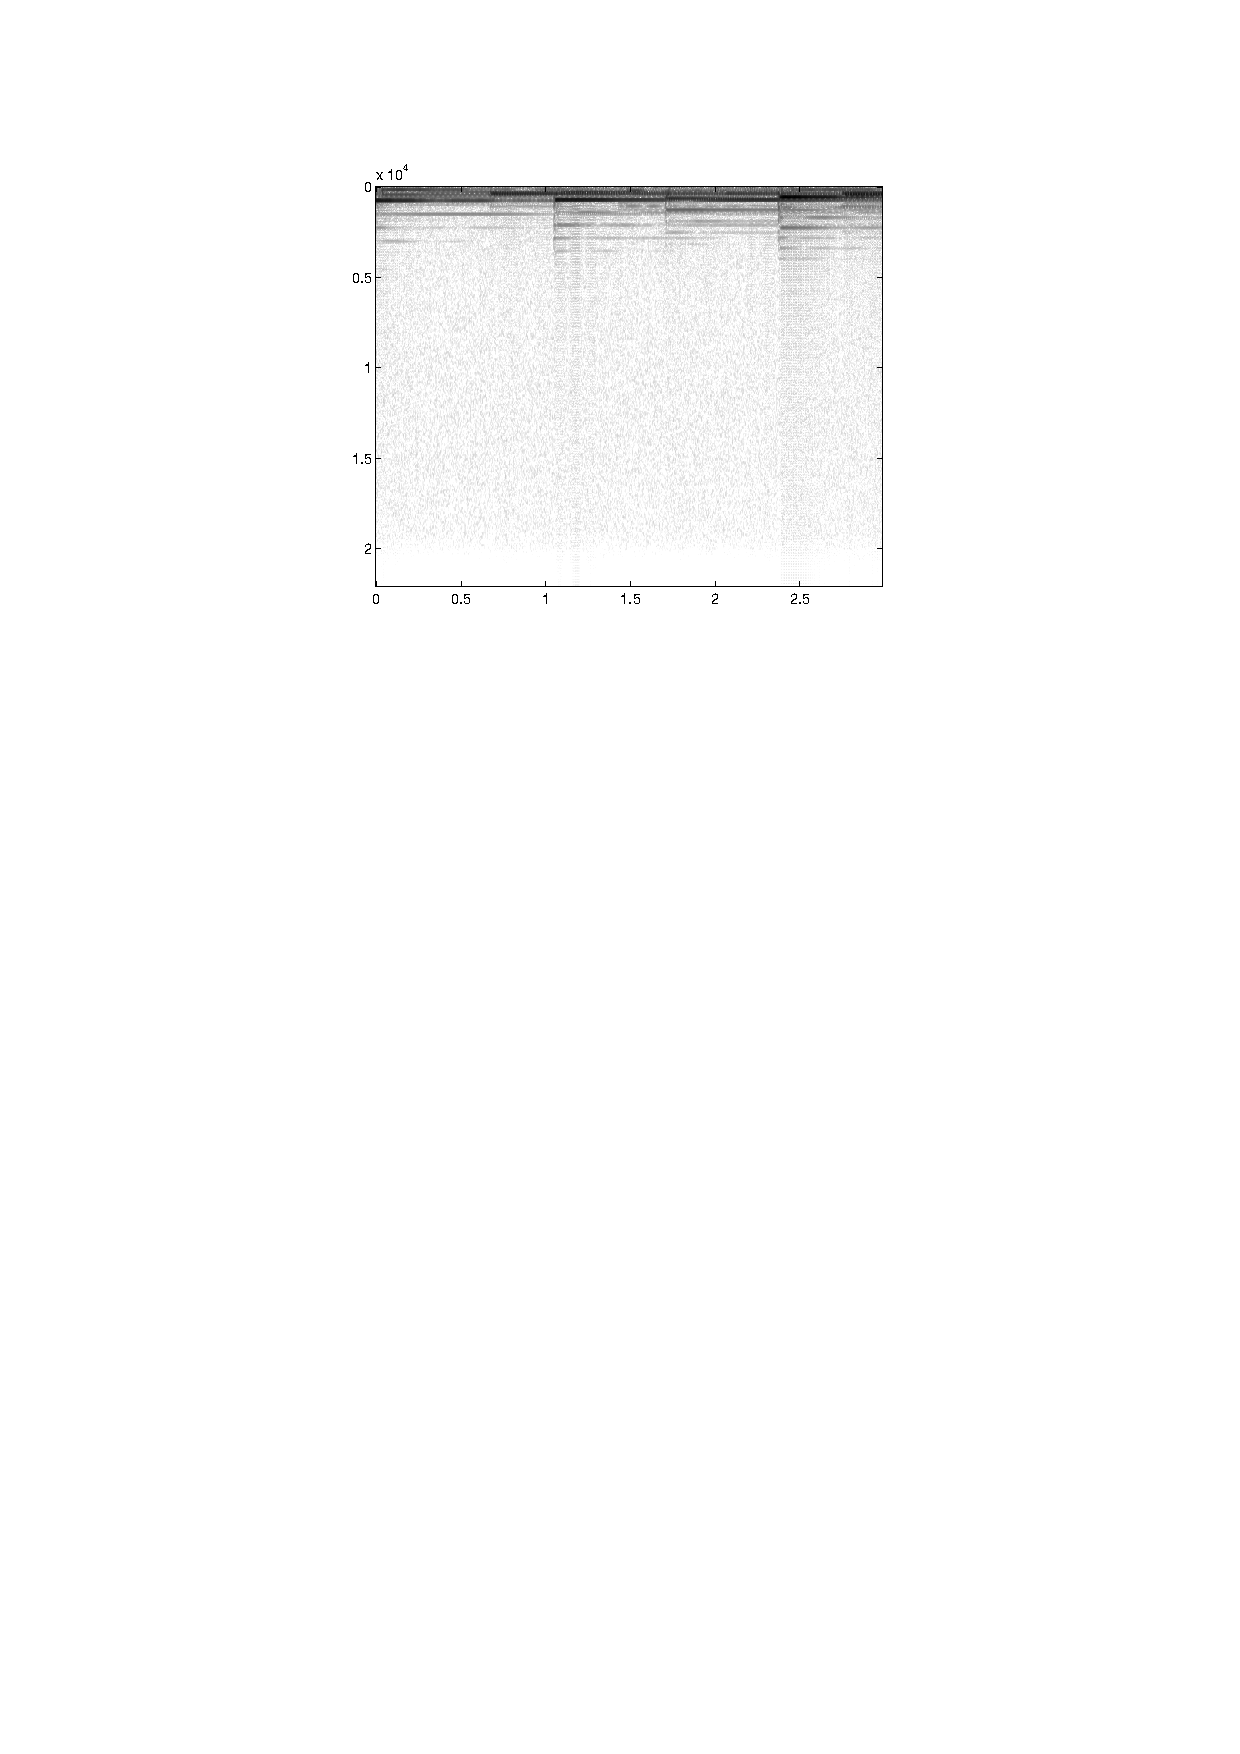
\includegraphics[width=0.6\textwidth]{Figures/Figure2-19}\\
  \caption{Spectrogramme d'un morceau de piano. On voit se succ\'{e}der les notes. Chaque note est caract\'{e}ris\'{e}e par l'apparition de raies qui s'affaiblissent \`{a} mesure que le son s'att\'{e}nue. (l'\'{e}chelle des fr\'{e}quences est du haut vers le bas et en $10000$ Hz d'unit\'{e}}\label{fig:figure2-19}
\end{figure}



\begin{figure}
  \centering
  % Requires \usepackage{graphicx}
  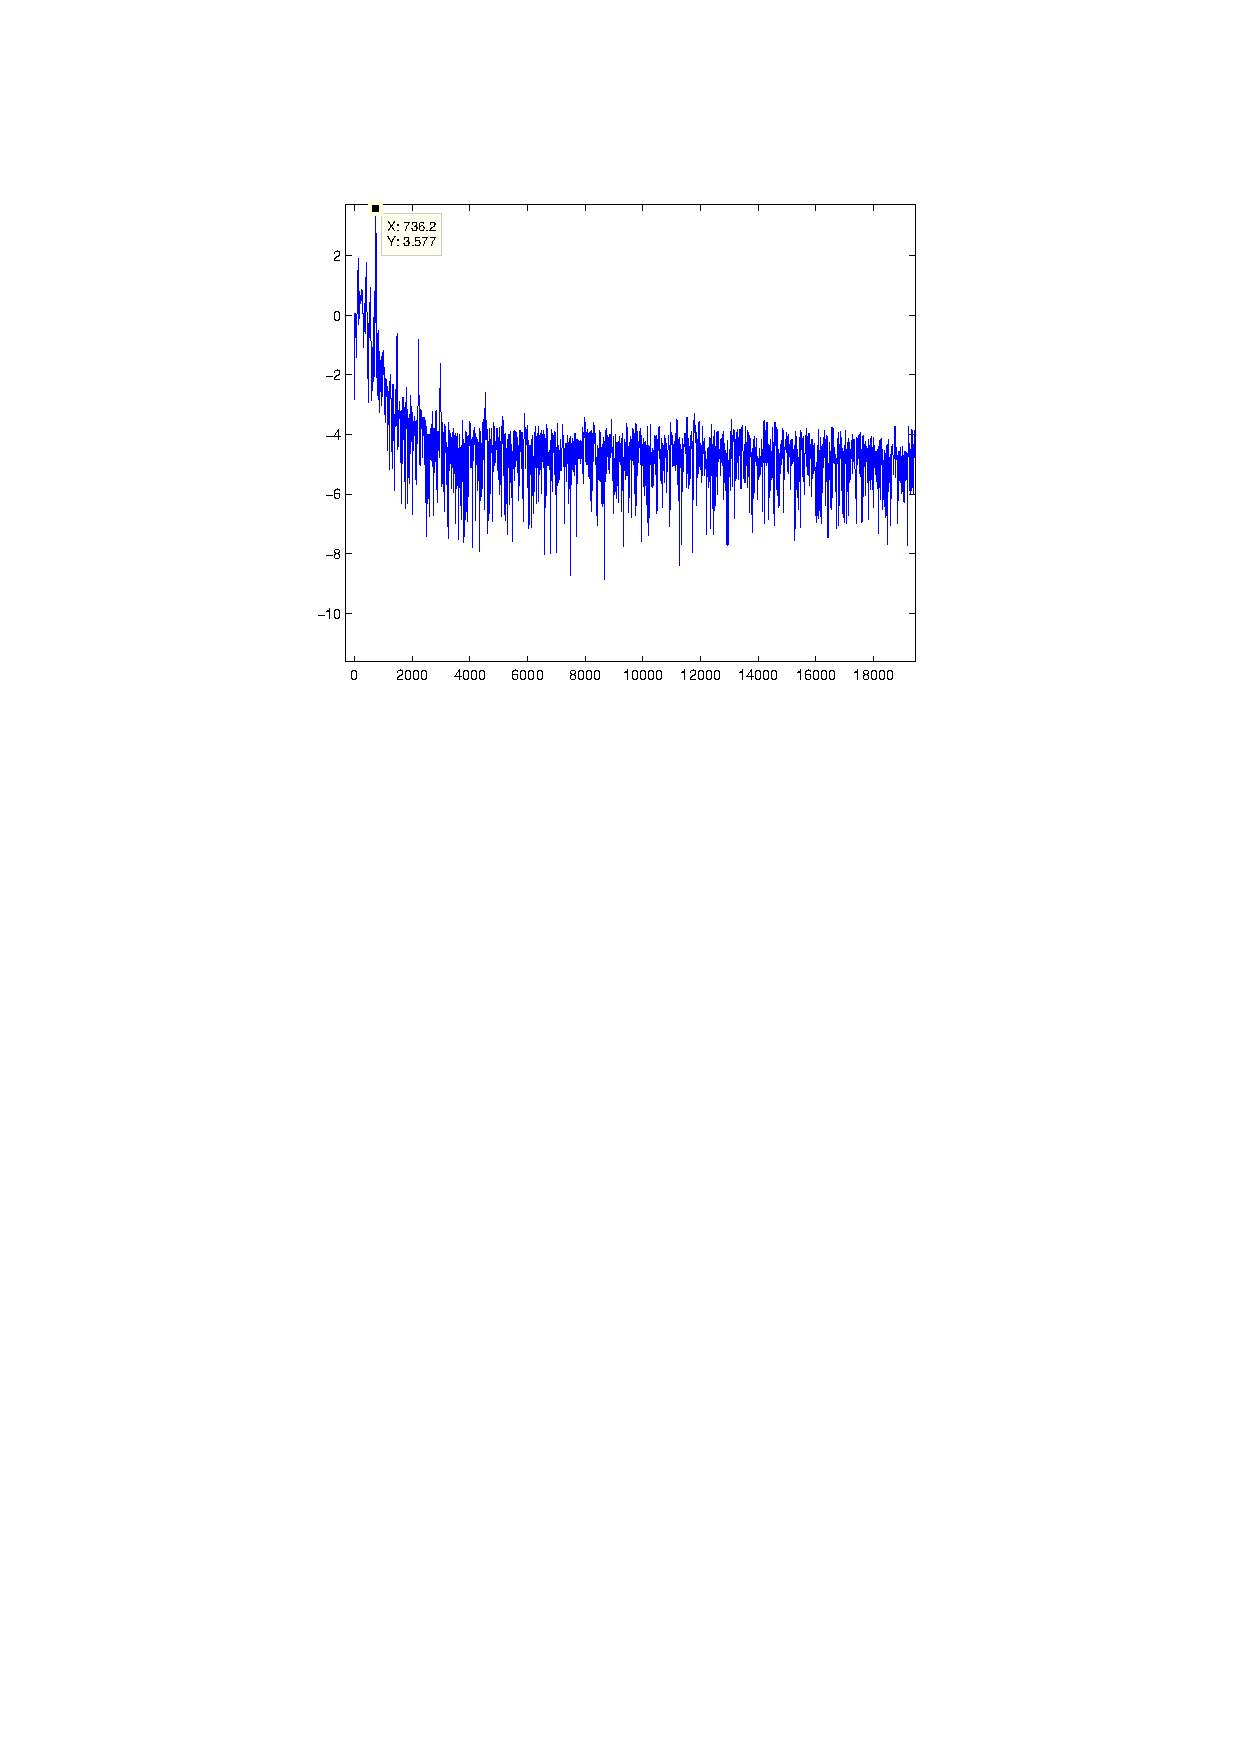
\includegraphics[width=0.6\textwidth]{Figures/Figure2-20}\\
  \caption{Une colonne du spectrogramme. C'est donc le contenu fr\'{e}quentiel local autour d'un certain instant. Le pic le plus pro\'{e}minent est pour la fr\'{e}quence $736$ Hz, qui correspond \`{a} peu pr\`{e}s \`{a} un Fa di\`{e}se.}\label{fig:figure2-20}
\end{figure}

